\section*{Глава 3. Реализация веб-приложения}
\addcontentsline{toc}{section}{Глава 3. Реализация веб-приложения}
\stepcounter{section}

% ----------------------------------------------------------------
\subsection{Структура проекта и основные файлы}
% ----------------------------------------------------------------

Проект организован как монорепозиторий, содержащий два независимых
приложения: серверную часть (\textit{backend}) и клиентскую часть
(\textit{frontend}). Разделение на два самостоятельных пакета позволяет
разрабатывать и развёртывать части системы независимо друг от друга.

Общая структура проекта представлена в листинге~\ref{lst:dirtree}.

\begin{lstlisting}[caption={Структура монорепозитория},
                   label=lst:dirtree]
table-time-app/
|-- backend/                    # NestJS API-сервер
|   |-- prisma/
|   |   |-- migrations/         # История миграций базы данных
|   |   |-- schema.prisma       # Схема модели данных
|   |   `-- seed.ts             # Скрипт начального заполнения БД
|   `-- src/
|       |-- main.ts             # Точка входа приложения
|       |-- app.module.ts       # Корневой модуль NestJS
|       |-- auth/               # Модуль аутентификации
|       |-- users/              # Модуль пользователей
|       |-- restaurants/        # Модуль ресторанов
|       |-- tables/             # Модуль столов и статусов
|       |-- menu/               # Модуль меню
|       |-- reservations/       # Модуль бронирований
|       |-- orders/             # Модуль заказов
|       |-- prisma/             # Обёртка над Prisma Client
|       `-- common/             # Общие фильтры, интерцепторы, утилиты
`-- frontend/                   # Next.js клиент
    `-- src/
        |-- app/                # Страницы (App Router)
        |   |-- page.tsx        # Главная страница
        |   |-- layout.tsx      # Корневой макет
        |   |-- login/          # Страница входа
        |   |-- register/       # Страница регистрации
        |   |-- menu/           # Страница меню
        |   |-- tables/         # Страница бронирования столов
        |   |-- order/          # Оформление заказа
        |   |-- orders/         # История заказов
        |   |-- me/             # Личный кабинет
        |   |-- staff/          # Страница официанта
        |   `-- admin/          # Административная панель
        |-- components/
        |   |-- Navbar.tsx      # Навигационная панель
        |   `-- ProtectedPage.tsx
        |-- contexts/
        |   |-- AuthContext.tsx
        |   |-- CartContext.tsx
        |   |-- LocaleContext.tsx
        |   `-- ToastContext.tsx
        |-- hooks/
        |-- lib/
        |   `-- i18n/           # Переводы (ru.ts, en.ts, types.ts)
        `-- shared/api/
            `-- client.ts       # HTTP-клиент (apiFetch, ApiError)
\end{lstlisting}

Каждый модуль серверной части следует единообразной структуре: контроллер
принимает HTTP-запросы и делегирует обработку сервису, сервис содержит
бизнес-логику и обращается к репозиторию или напрямую к Prisma.
DTO-файлы описывают структуру входных данных и правила их валидации.

На стороне фронтенда используется App Router Next.js~15: каждая папка
в \texttt{app/} соответствует маршруту, а файл \texttt{page.tsx}~---
компоненту страницы. Общие контексты (\texttt{AuthContext},
\texttt{LocaleContext}) оборачивают всё дерево компонентов через корневой
\texttt{layout.tsx}. HTTP-взаимодействие с бэкендом централизовано
в функции \texttt{apiFetch} из \texttt{shared/api/client.ts}, которая
единообразно обрабатывает ошибки и бросает типизированный
\texttt{ApiError}.

% ----------------------------------------------------------------
\subsection{Реализация модели данных}
% ----------------------------------------------------------------

Для хранения данных используется СУБД PostgreSQL. Работа с базой данных
осуществляется через ORM Prisma, которая обеспечивает типобезопасный
доступ к данным и управление схемой через декларативный файл
\texttt{schema.prisma}.

Схема содержит восемь таблиц и шесть перечислений (\textit{enum}).
Ниже описаны все сущности модели данных.

\textbf{Перечисления}

В схеме определены следующие перечисления:
\begin{itemize}
  \item \textbf{Role}~--- роль пользователя: \texttt{GUEST},
        \texttt{USER}, \texttt{WAITER}, \texttt{ADMIN};
  \item \textbf{TableStatus}~--- статус стола: \texttt{FREE},
        \texttt{RESERVED}, \texttt{OCCUPIED}, \texttt{CLEANING};
  \item \textbf{DishCategory}~--- категория блюда:
        \texttt{hot\_drinks}, \texttt{cold\_drinks},
        \texttt{breakfast}, \texttt{sandwiches}, \texttt{main},
        \texttt{salads}, \texttt{desserts}, \texttt{signature};
  \item \textbf{OrderType}~--- тип заказа: \texttt{DINE\_IN},
        \texttt{DELIVERY}, \texttt{TAKEAWAY};
  \item \textbf{OrderStatus}~--- статус заказа: \texttt{CREATED},
        \texttt{CONFIRMED}, \texttt{PREPARING}, \texttt{READY},
        \texttt{COMPLETED}, \texttt{CANCELLED};
  \item \textbf{ReservationStatus}~--- статус бронирования:
        \texttt{PENDING}, \texttt{CONFIRMED}, \texttt{CANCELLED},
        \texttt{COMPLETED};
  \item \textbf{PaymentMethod}~--- способ оплаты: \texttt{CASH},
        \texttt{CARD}.
\end{itemize}

\textbf{Сущность User (пользователи)}

Таблица \texttt{users} хранит учётные записи всех пользователей системы.
Основные поля: уникальный идентификатор (UUID), электронная почта
(уникальная), хэш пароля, роль и временные метки создания и обновления.
Пароли хранятся в виде хэша, полученного алгоритмом Argon2.

\textbf{Сущность RefreshToken (токены обновления)}

Таблица \texttt{refresh\_tokens} хранит хэши выданных refresh-токенов
с привязкой к пользователю и датой истечения срока действия. Хранение
хэша (а не самого токена) позволяет инвалидировать конкретную сессию
без компрометации других. При выходе из системы все токены пользователя
удаляются.

\textbf{Сущность Restaurant (ресторан)}

Таблица \texttt{restaurants} содержит информацию о заведении: название,
адрес и описание. Архитектурно предусмотрена поддержка нескольких
ресторанов, однако в текущей реализации используется одна запись.

\textbf{Сущность Table (столы)}

Таблица \texttt{tables} описывает столы заведения. Каждый стол
принадлежит ресторану, имеет номер, вместимость и координаты на карте
зала (поля \texttt{x} и \texttt{y} в процентах). Статус стола хранится
денормализованно как вспомогательный отображаемый атрибут. Актуальная
доступность при бронировании определяется запросом к таблице
\texttt{reservations}. Поля \texttt{cleaningStartedAt} и
\texttt{statusExpiresAt} используются системой автоматических таймеров
для восстановления состояния после перезапуска сервера. Стол может быть
назначен официанту через связь \texttt{assignedWaiterId}.

\textbf{Сущность Dish (блюда)}

Таблица \texttt{dishes} хранит позиции меню. Каждое блюдо имеет название
на русском и английском языках, цену, категорию, путь к изображению и
признак доступности \texttt{isAvailable}. Удаление блюда из меню
реализовано как мягкое: запись остаётся в базе, но поле
\texttt{isAvailable} устанавливается в \texttt{false}.

\textbf{Сущность Order (заказы)}

Таблица \texttt{orders} хранит заказы пользователей. Заказ связан
с пользователем, опционально~--- со столом и бронированием. Тип заказа
определяет, какие поля являются обязательными: для \texttt{DINE\_IN}~---
стол, для \texttt{DELIVERY}~--- адрес доставки. Поле \texttt{scheduledAt}
позволяет оформить предварительный заказ к указанному времени. Общая
сумма вычисляется на основе позиций и фиксируется в поле
\texttt{totalAmount}.

\textbf{Сущность OrderItem (позиции заказа)}

Таблица \texttt{order\_items} хранит отдельные позиции заказа с привязкой
к блюду и количеством. Поле \texttt{unitPrice} фиксирует цену блюда на
момент оформления заказа~--- это исключает влияние последующих изменений
цен на историю заказов.

\textbf{Сущность Reservation (бронирования)}

Таблица \texttt{reservations} хранит бронирования столов. Каждое
бронирование связано с пользователем, столом и рестораном, содержит
время начала и окончания визита и количество гостей. Проверка на конфликт
бронирований выполняется на уровне сервиса по условию перекрытия
временных интервалов. Для поддержки этого запроса предусмотрен составной
индекс по полям \texttt{tableId}, \texttt{startTime}, \texttt{endTime}.


% ----------------------------------------------------------------
\subsection{Миграции базы данных}
% ----------------------------------------------------------------

Управление схемой базы данных осуществляется через систему миграций
Prisma Migrate. Каждая миграция представляет собой SQL-файл,
автоматически сгенерированный на основе изменений в
\texttt{schema.prisma}. Миграции применяются командой
\texttt{prisma migrate deploy} и фиксируются в системе контроля версий
вместе с кодом приложения.

В ходе разработки проекта было создано семь миграций, каждая из которых
соответствует определённому этапу эволюции схемы.

\textbf{Миграция~1~--- init (25.04.2026)}

Начальная миграция создаёт базовую структуру приложения: таблицы
\texttt{users}, \texttt{refresh\_tokens}, \texttt{restaurants},
\texttt{tables}, \texttt{dishes}, \texttt{orders},
\texttt{order\_items}, \texttt{reservations}. Определяются все
перечисления, первичные ключи, внешние ключи и индексы.
Устанавливаются ограничения ссылочной целостности.

\textbf{Миграция~2~--- add\_reservation\_status (25.04.2026)}

Добавляет перечисление \texttt{ReservationStatus} (\texttt{PENDING},
\texttt{CONFIRMED}, \texttt{CANCELLED}, \texttt{COMPLETED}) и одноимённое
поле в таблицу \texttt{reservations} со значением по умолчанию
\texttt{PENDING}. Вводит жизненный цикл бронирования, управляемый
статусами.

\textbf{Миграция~3~--- add\_missing\_order\_fields (27.04.2026)}

Расширяет таблицу \texttt{orders} полями: \texttt{scheduledAt}
(дата и время предварительного заказа), \texttt{deliveryAddress}
(адрес доставки), \texttt{reservationId} (связь с бронированием) и
\texttt{paymentMethod} (перечисление \texttt{PaymentMethod}).
Добавляются соответствующие индексы.

\textbf{Миграция~4~--- add\_table\_number (27.04.2026)}

Добавляет в таблицу \texttt{tables} поле \texttt{number}~--- номер
стола, отображаемый в интерфейсе. До этого столы идентифицировались
только по UUID.

\textbf{Миграция~5~--- phase3\_dish\_i18n\_payment\_waiter\_assign
(16.05.2026)}

Комплексное обновление третьего этапа разработки. В таблицу
\texttt{dishes} добавляется поле \texttt{nameEn} для хранения
английского названия блюда. В таблицу \texttt{tables} добавляется поле
\texttt{assignedWaiterId} с внешним ключом на таблицу \texttt{users},
реализующее назначение официанта на стол.

\textbf{Миграция~6~--- add\_cleaning\_started\_at (06.06.2026)}

Добавляет в таблицу \texttt{tables} поле \texttt{cleaningStartedAt}~---
метку времени начала уборки. Поле используется при перезапуске сервера
для вычисления оставшегося времени уборки и восстановления активных
таймеров.

\textbf{Миграция~7~--- add\_status\_expires\_at (06.06.2026)}

Добавляет в таблицу \texttt{tables} поле \texttt{statusExpiresAt}~---
унифицированный момент истечения любого временного статуса
(\texttt{CLEANING}, \texttt{OCCUPIED}, \texttt{RESERVED}). Поле
позволяет фронтенду отображать актуальный статус в реальном времени
без дополнительных запросов к серверу.

Совместное применение полей \texttt{cleaningStartedAt} и
\texttt{statusExpiresAt} обеспечивает устойчивость системы статусов
к перезапускам сервера: при старте метод \texttt{onModuleInit}
восстанавливает все активные таймеры по данным из базы.

% ----------------------------------------------------------------
\subsection{Реализация REST API}
% ----------------------------------------------------------------

Серверная часть предоставляет REST API с глобальным префиксом
\texttt{/api}. Маршруты организованы по ресурсам и защищены на уровне
контроллеров с помощью guards: \texttt{JwtAuthGuard} проверяет наличие
действующего access-токена, \texttt{RolesGuard}~--- соответствие роли
пользователя требуемой.

Входные данные валидируются глобальным \texttt{ValidationPipe}
с параметрами \texttt{whitelist: true} и \texttt{transform: true}:
неизвестные поля отбрасываются, а строковые query-параметры
автоматически преобразуются к нужным типам. Все HTTP-ошибки
нормализуются глобальным \texttt{HttpExceptionFilter} и возвращаются
клиенту в единообразном формате \texttt{\{statusCode, message\}}.
Каждый запрос и ответ протоколируются через \texttt{LoggingInterceptor}.

Ниже приведены все доступные эндпоинты, сгруппированные по модулям.

\begin{table}[H]
\centering
\caption{Эндпоинты модуля Auth (\texttt{/api/auth})}
\label{tab:api_auth}
\begin{tabular}{|p{1.4cm}|p{5.8cm}|p{2.6cm}|p{4.8cm}|}
\hline
\textbf{Метод} & \textbf{Маршрут} & \textbf{Доступ} &
\textbf{Описание} \\
\hline
POST & /api/auth/register & Публичный &
  Регистрация нового пользователя \\ \hline
POST & /api/auth/login    & Публичный &
  Вход в систему \\ \hline
POST & /api/auth/refresh  & refresh-токен &
  Обновление пары токенов \\ \hline
POST & /api/auth/logout   & Авторизован &
  Выход, удаление токенов \\ \hline
\end{tabular}
\end{table}

\begin{table}[H]
\centering
\caption{Эндпоинты модуля Users (\texttt{/api/users})}
\label{tab:api_users}
\begin{tabular}{|p{1.8cm}|p{5.4cm}|p{2.6cm}|p{4.8cm}|}
\hline
\textbf{Метод} & \textbf{Маршрут} & \textbf{Доступ} &
\textbf{Описание} \\
\hline
GET    & /api/users/me        & Авторизован &
  Профиль текущего пользователя \\ \hline
GET    & /api/users           & ADMIN &
  Список всех пользователей \\ \hline
GET    & /api/users/:id       & ADMIN &
  Пользователь по ID \\ \hline
POST   & /api/users           & ADMIN &
  Создание аккаунта сотрудника \\ \hline
PATCH  & /api/users/:id/role  & ADMIN &
  Изменение роли пользователя \\ \hline
DELETE & /api/users/:id       & ADMIN &
  Удаление аккаунта \\ \hline
\end{tabular}
\end{table}

\begin{table}[H]
\centering
\caption{Эндпоинты модуля Restaurants (\texttt{/api/restaurants})}
\label{tab:api_restaurants}
\begin{tabular}{|p{1.4cm}|p{5.8cm}|p{2.6cm}|p{4.8cm}|}
\hline
\textbf{Метод} & \textbf{Маршрут} & \textbf{Доступ} &
\textbf{Описание} \\
\hline
GET   & /api/restaurants     & Публичный &
  Список ресторанов \\ \hline
GET   & /api/restaurants/:id & Публичный &
  Ресторан по ID \\ \hline
POST  & /api/restaurants     & ADMIN &
  Создание ресторана \\ \hline
PATCH & /api/restaurants/:id & ADMIN &
  Редактирование ресторана \\ \hline
\end{tabular}
\end{table}

\begin{table}[H]
\centering
\caption{Эндпоинты модуля Tables (\texttt{/api/tables})}
\label{tab:api_tables}
\begin{tabular}{|p{1.4cm}|p{5.8cm}|p{2.6cm}|p{4.8cm}|}
\hline
\textbf{Метод} & \textbf{Маршрут} & \textbf{Доступ} &
\textbf{Описание} \\
\hline
GET   & /api/tables                & Публичный &
  Список всех столов \\ \hline
GET   & /api/tables/:id            & Публичный &
  Стол по ID \\ \hline
POST  & /api/tables                & ADMIN &
  Создание стола \\ \hline
PATCH & /api/tables/:id            & ADMIN &
  Редактирование параметров стола \\ \hline
PATCH & /api/tables/:id/status     & ADMIN &
  Ручное изменение статуса \\ \hline
PATCH & /api/tables/:id/assign     & ADMIN &
  Назначение/снятие официанта \\ \hline
\end{tabular}
\end{table}

\begin{table}[H]
\centering
\caption{Эндпоинты модуля Menu (\texttt{/api/menu})}
\label{tab:api_menu}
\begin{tabular}{|p{1.8cm}|p{5.4cm}|p{2.6cm}|p{4.8cm}|}
\hline
\textbf{Метод} & \textbf{Маршрут} & \textbf{Доступ} &
\textbf{Описание} \\
\hline
GET    & /api/menu           & Публичный &
  Доступные блюда (с фильтром по категории) \\ \hline
GET    & /api/menu/admin/all & ADMIN &
  Все блюда, включая недоступные \\ \hline
GET    & /api/menu/:id       & Публичный &
  Блюдо по ID \\ \hline
POST   & /api/menu           & ADMIN &
  Создание блюда \\ \hline
PATCH  & /api/menu/:id       & ADMIN &
  Редактирование блюда \\ \hline
DELETE & /api/menu/:id       & ADMIN &
  Мягкое удаление (\texttt{isAvailable = false}) \\ \hline
\end{tabular}
\end{table}
\begin{table}[H]
\centering
\caption{Эндпоинты модуля Reservations (\texttt{/api/reservations})}
\label{tab:api_reservations}
\begin{tabular}{|p{1.4cm}|p{5.8cm}|p{2.6cm}|p{4.8cm}|}
\hline
\textbf{Метод} & \textbf{Маршрут} & \textbf{Доступ} &
\textbf{Описание} \\
\hline
POST  & /api/reservations                  & Авторизован &
  Создание бронирования \\ \hline
GET   & /api/reservations/available        & Публичный &
  Доступные столы для временного слота \\ \hline
GET   & /api/reservations/me               & Авторизован &
  Бронирования текущего пользователя \\ \hline
GET   & /api/reservations/restaurant/:id   & WAITER, ADMIN &
  Все бронирования ресторана \\ \hline
PATCH & /api/reservations/:id/cancel       & Авторизован &
  Отмена бронирования \\ \hline
PATCH & /api/reservations/:id/confirm      & WAITER, ADMIN &
  Подтверждение бронирования \\ \hline
PATCH & /api/reservations/:id/complete     & WAITER, ADMIN &
  Завершение бронирования \\ \hline
\end{tabular}
\end{table}

\begin{table}[H]
\centering
\caption{Эндпоинты модуля Orders (\texttt{/api/orders})}
\label{tab:api_orders}
\begin{tabular}{|p{1.8cm}|p{5.4cm}|p{2.9cm}|p{4.8cm}|}
\hline
\textbf{Метод} & \textbf{Маршрут} & \textbf{Доступ} &
\textbf{Описание} \\
\hline
GET    & /api/orders/me                  & Авторизован &
  Заказы текущего пользователя \\ \hline
GET    & /api/orders/table/:tableId      & WAITER, ADMIN &
  Активный заказ за столом \\ \hline
GET    & /api/orders                     & WAITER, ADMIN &
  Все заказы (с фильтрацией и пагинацией) \\ \hline
GET    & /api/orders/:id                 & Авторизован+ &
  Заказ по ID \\ \hline
POST   & /api/orders                     & Авторизован &
  Создание черновика заказа \\ \hline
POST   & /api/orders/:id/items           & Авторизован+ &
  Добавление позиции в заказ \\ \hline
DELETE & /api/orders/:id/items/:itemId   & Авторизован+ &
  Удаление позиции из заказа \\ \hline
PATCH  & /api/orders/:id/place           & Авторизован+ &
  Отправка заказа (\texttt{CREATED} $\to$ \texttt{CONFIRMED}) \\ \hline
PATCH  & /api/orders/:id/status          & WAITER, ADMIN &
  Переход к следующему статусу \\ \hline
PATCH  & /api/orders/:id/cancel          & Авторизован+ &
  Отмена заказа \\ \hline
\multicolumn{4}{|l|}{\footnotesize
  Авторизован+~--- собственник заказа, WAITER или ADMIN
  (проверяется через \texttt{OrderAccessGuard})} \\ \hline
\end{tabular}
\end{table}

% ----------------------------------------------------------------
\subsection{Реализация системы аутентификации и авторизации}
% ----------------------------------------------------------------

Система аутентификации реализована на основе JWT-токенов,
передаваемых через HTTP-only куки. При входе пользователь получает
пару токенов: access-токен со временем жизни 15~минут и refresh-токен
сроком на 7~суток. Access-токен используется для авторизации запросов
к API, refresh-токен~--- для автоматического обновления сессии без
повторного ввода учётных данных.

В приложении реализованы четыре роли пользователей:
\begin{itemize}
  \item \texttt{GUEST}~--- незарегистрированный пользователь; имеет
        доступ к просмотру меню и карте столов;
  \item \texttt{USER}~--- зарегистрированный пользователь; может
        бронировать столы и оформлять заказы;
  \item \texttt{WAITER}~--- официант; получает доступ к управлению
        заказами за назначенными ему столами;
  \item \texttt{ADMIN}~--- администратор; имеет полный доступ ко всем
        разделам системы.
\end{itemize}

На фронтенде защита маршрутов реализована через компонент
\texttt{ProtectedPage}, который проверяет текущую роль пользователя
и перенаправляет на главную страницу при отсутствии необходимых прав
доступа.

Формы входа и регистрации реализованы на отдельных страницах.
Форма входа представлена на рисунке~\ref{fig:login}.

\begin{figure}[H]
\centering
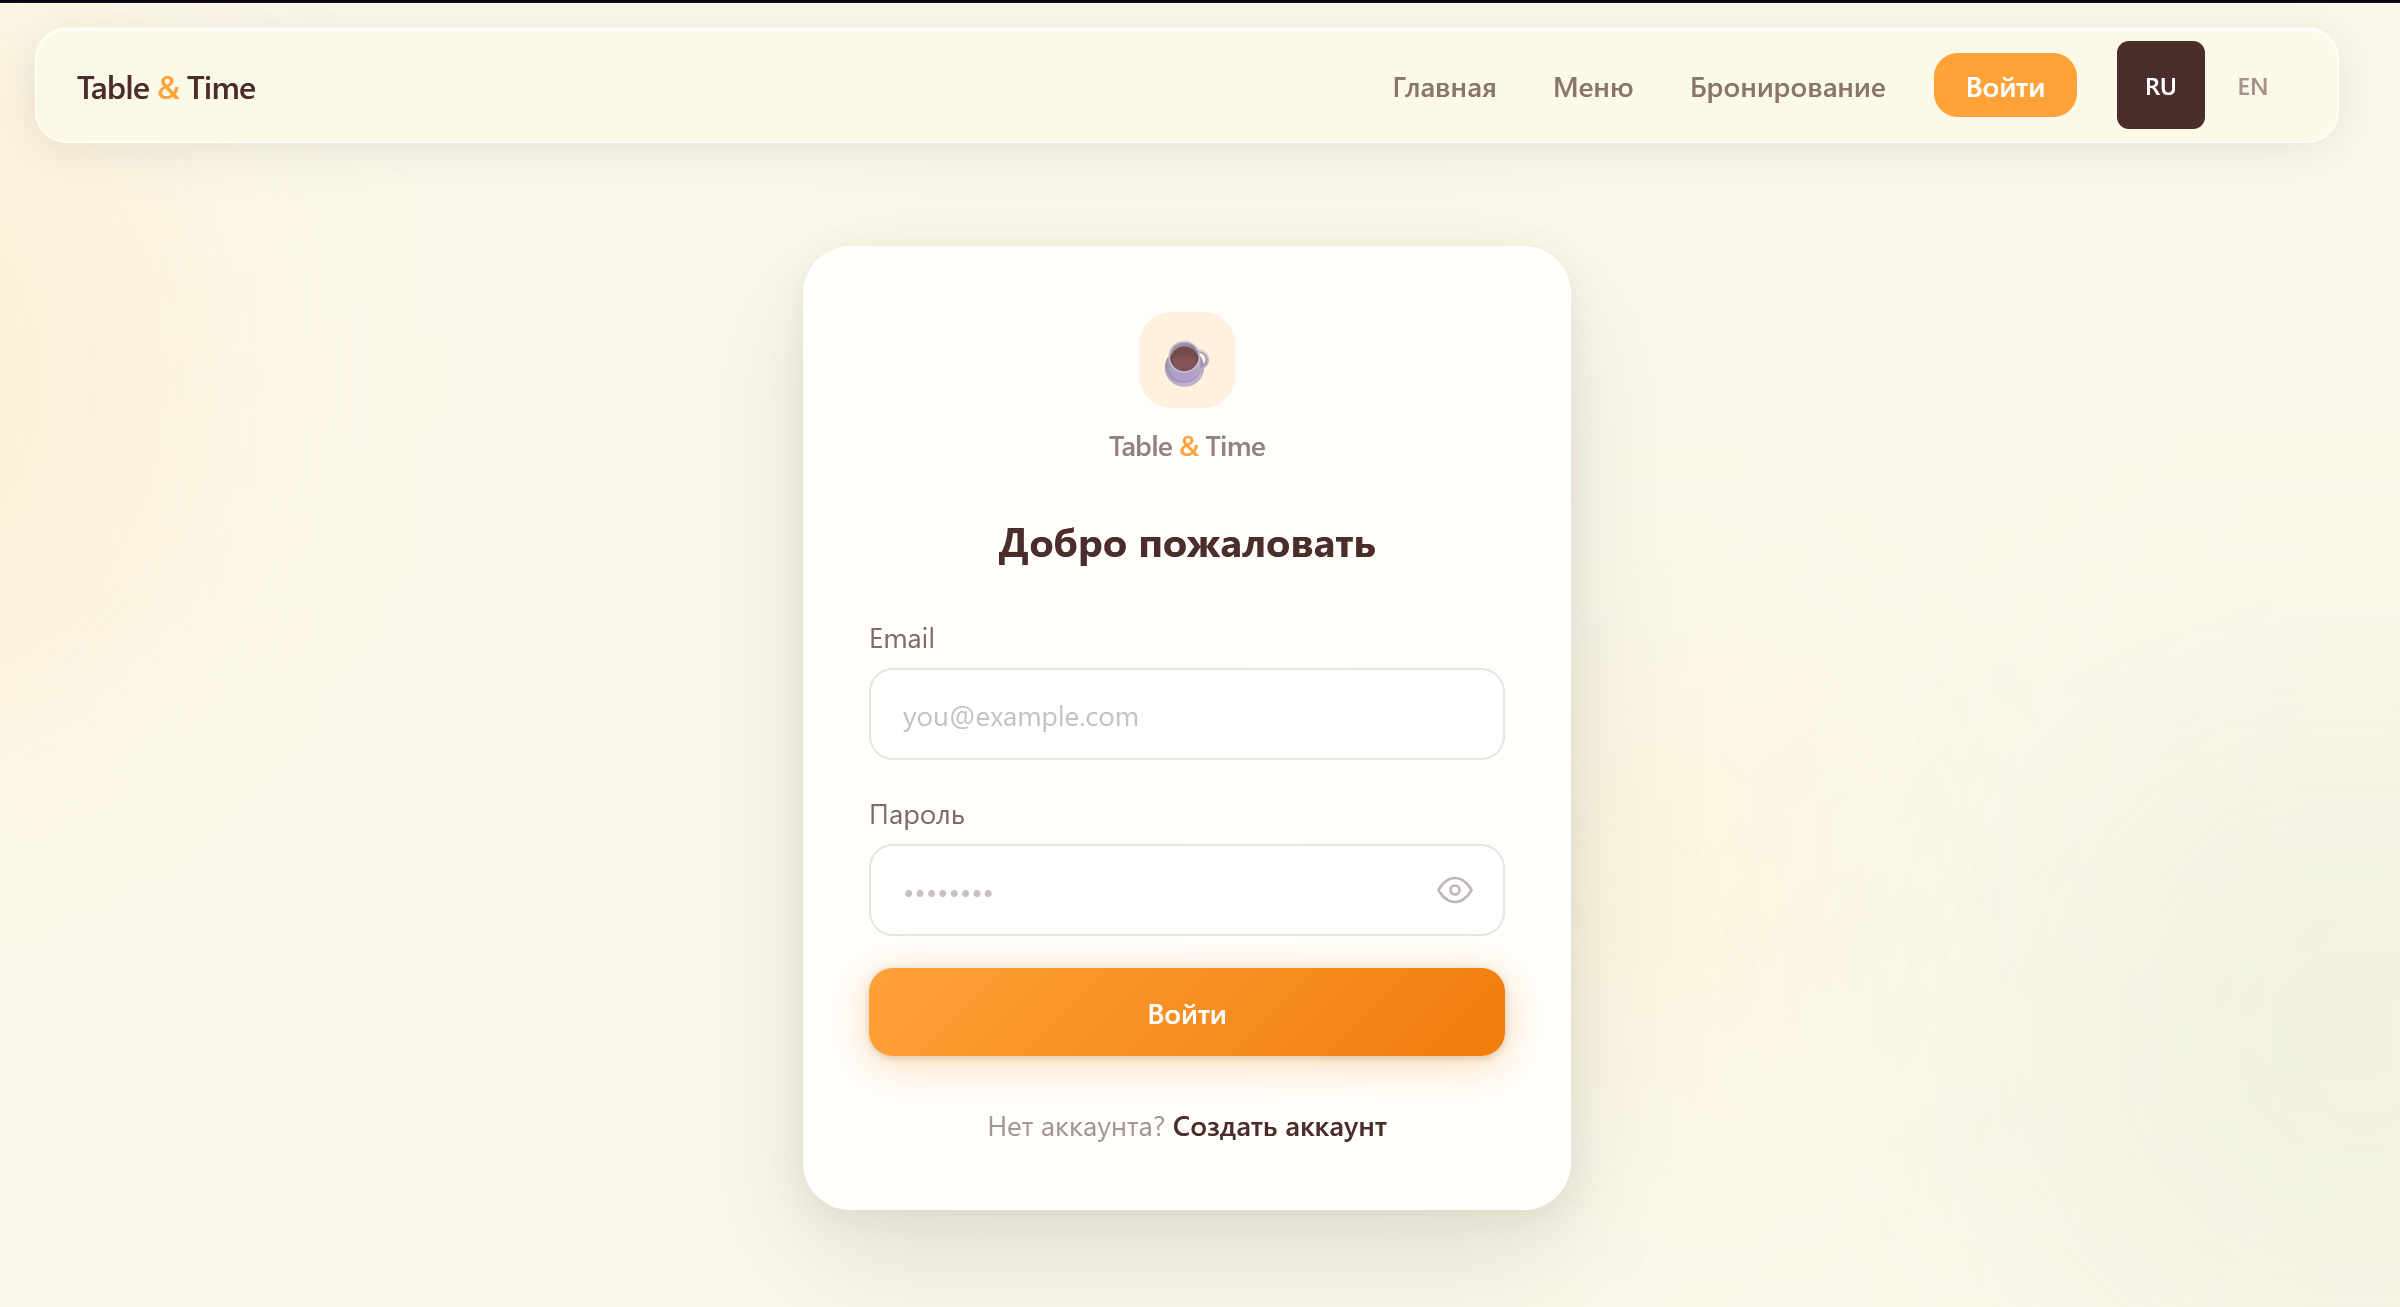
\includegraphics[width=0.85\textwidth]{images/login.png}
\caption{Форма входа в систему (страница \texttt{/login}):
         поле email, поле пароля, кнопка «Войти»,
         ссылка на регистрацию}
\label{fig:login}
\end{figure}

Форма регистрации включает поля электронной почты и пароля. После
успешной регистрации пользователю автоматически присваивается роль
\texttt{USER} и он перенаправляется в личный кабинет.

% ----------------------------------------------------------------
\subsection{Реализация главной страницы и навигации}
% ----------------------------------------------------------------

Навигационная панель отображается на всех страницах приложения и
адаптируется в зависимости от роли пользователя. Для гостя доступны
ссылки на главную страницу, меню, страницу столов, а также кнопки
входа и регистрации. Для авторизованного пользователя вместо них
отображается ссылка на личный кабинет и кнопка выхода из системы.
Для администратора добавляется ссылка на панель администрирования.

Навигационная панель зафиксирована в верхней части экрана и
перекрывает остальной контент, что обеспечивает постоянный доступ
к разделам при прокрутке страницы.

На главной странице отображается информация о заведении: название,
краткое описание концепции кафе и галерея изображений. Страница
создаёт первое впечатление о заведении и содержит призыв к
действию~--- кнопку перехода к бронированию стола.

\begin{figure}[H]
\centering
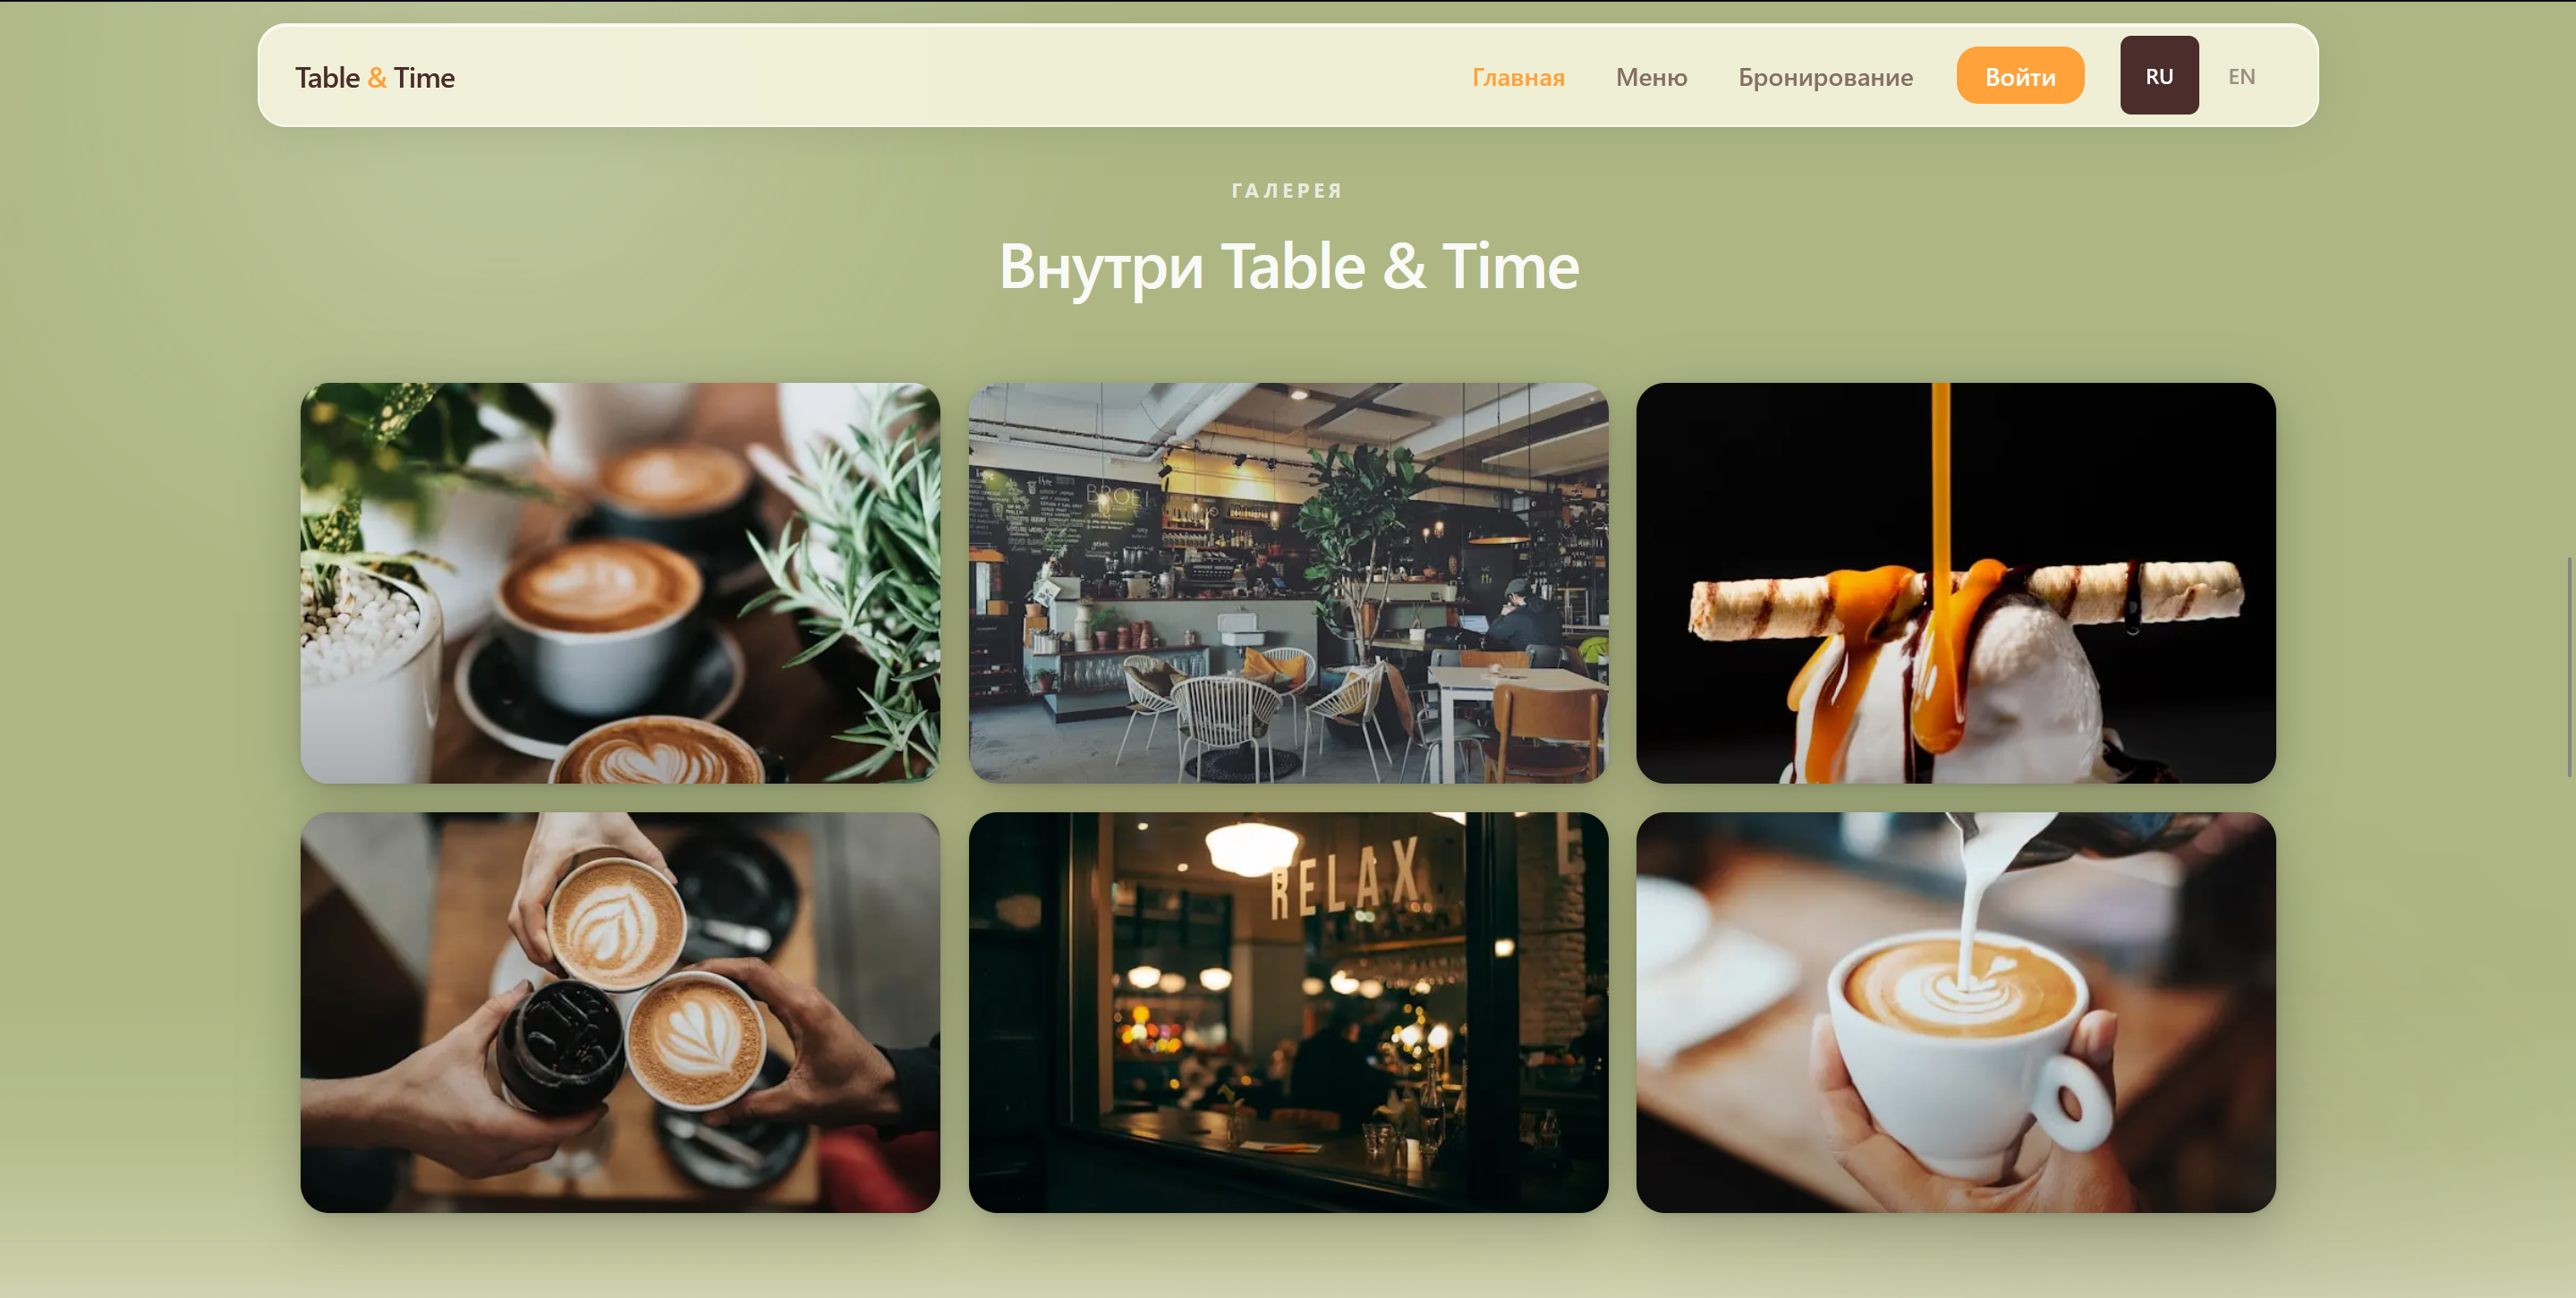
\includegraphics[width=0.85\textwidth]{images/main.png}
\caption{Главная страница приложения: шапка с навигацией,
         секция с описанием кафе, галерея изображений,
         кнопка «Забронировать стол»}
\label{fig:main}
\end{figure}

% ----------------------------------------------------------------
\subsection{Реализация страницы меню}
% ----------------------------------------------------------------

Страница меню отображает блюда и напитки кафе, разбитые по восьми
категориям: горячие напитки, холодные напитки, завтраки, сэндвичи,
основные блюда, салаты, десерты и фирменные блюда.

Пользователь может переключаться между категориями с помощью панели
фильтрации в верхней части страницы. При выборе категории
отображаются только позиции, относящиеся к ней. Каждая карточка
блюда содержит изображение, название и цену.

\begin{figure}[H]
\centering
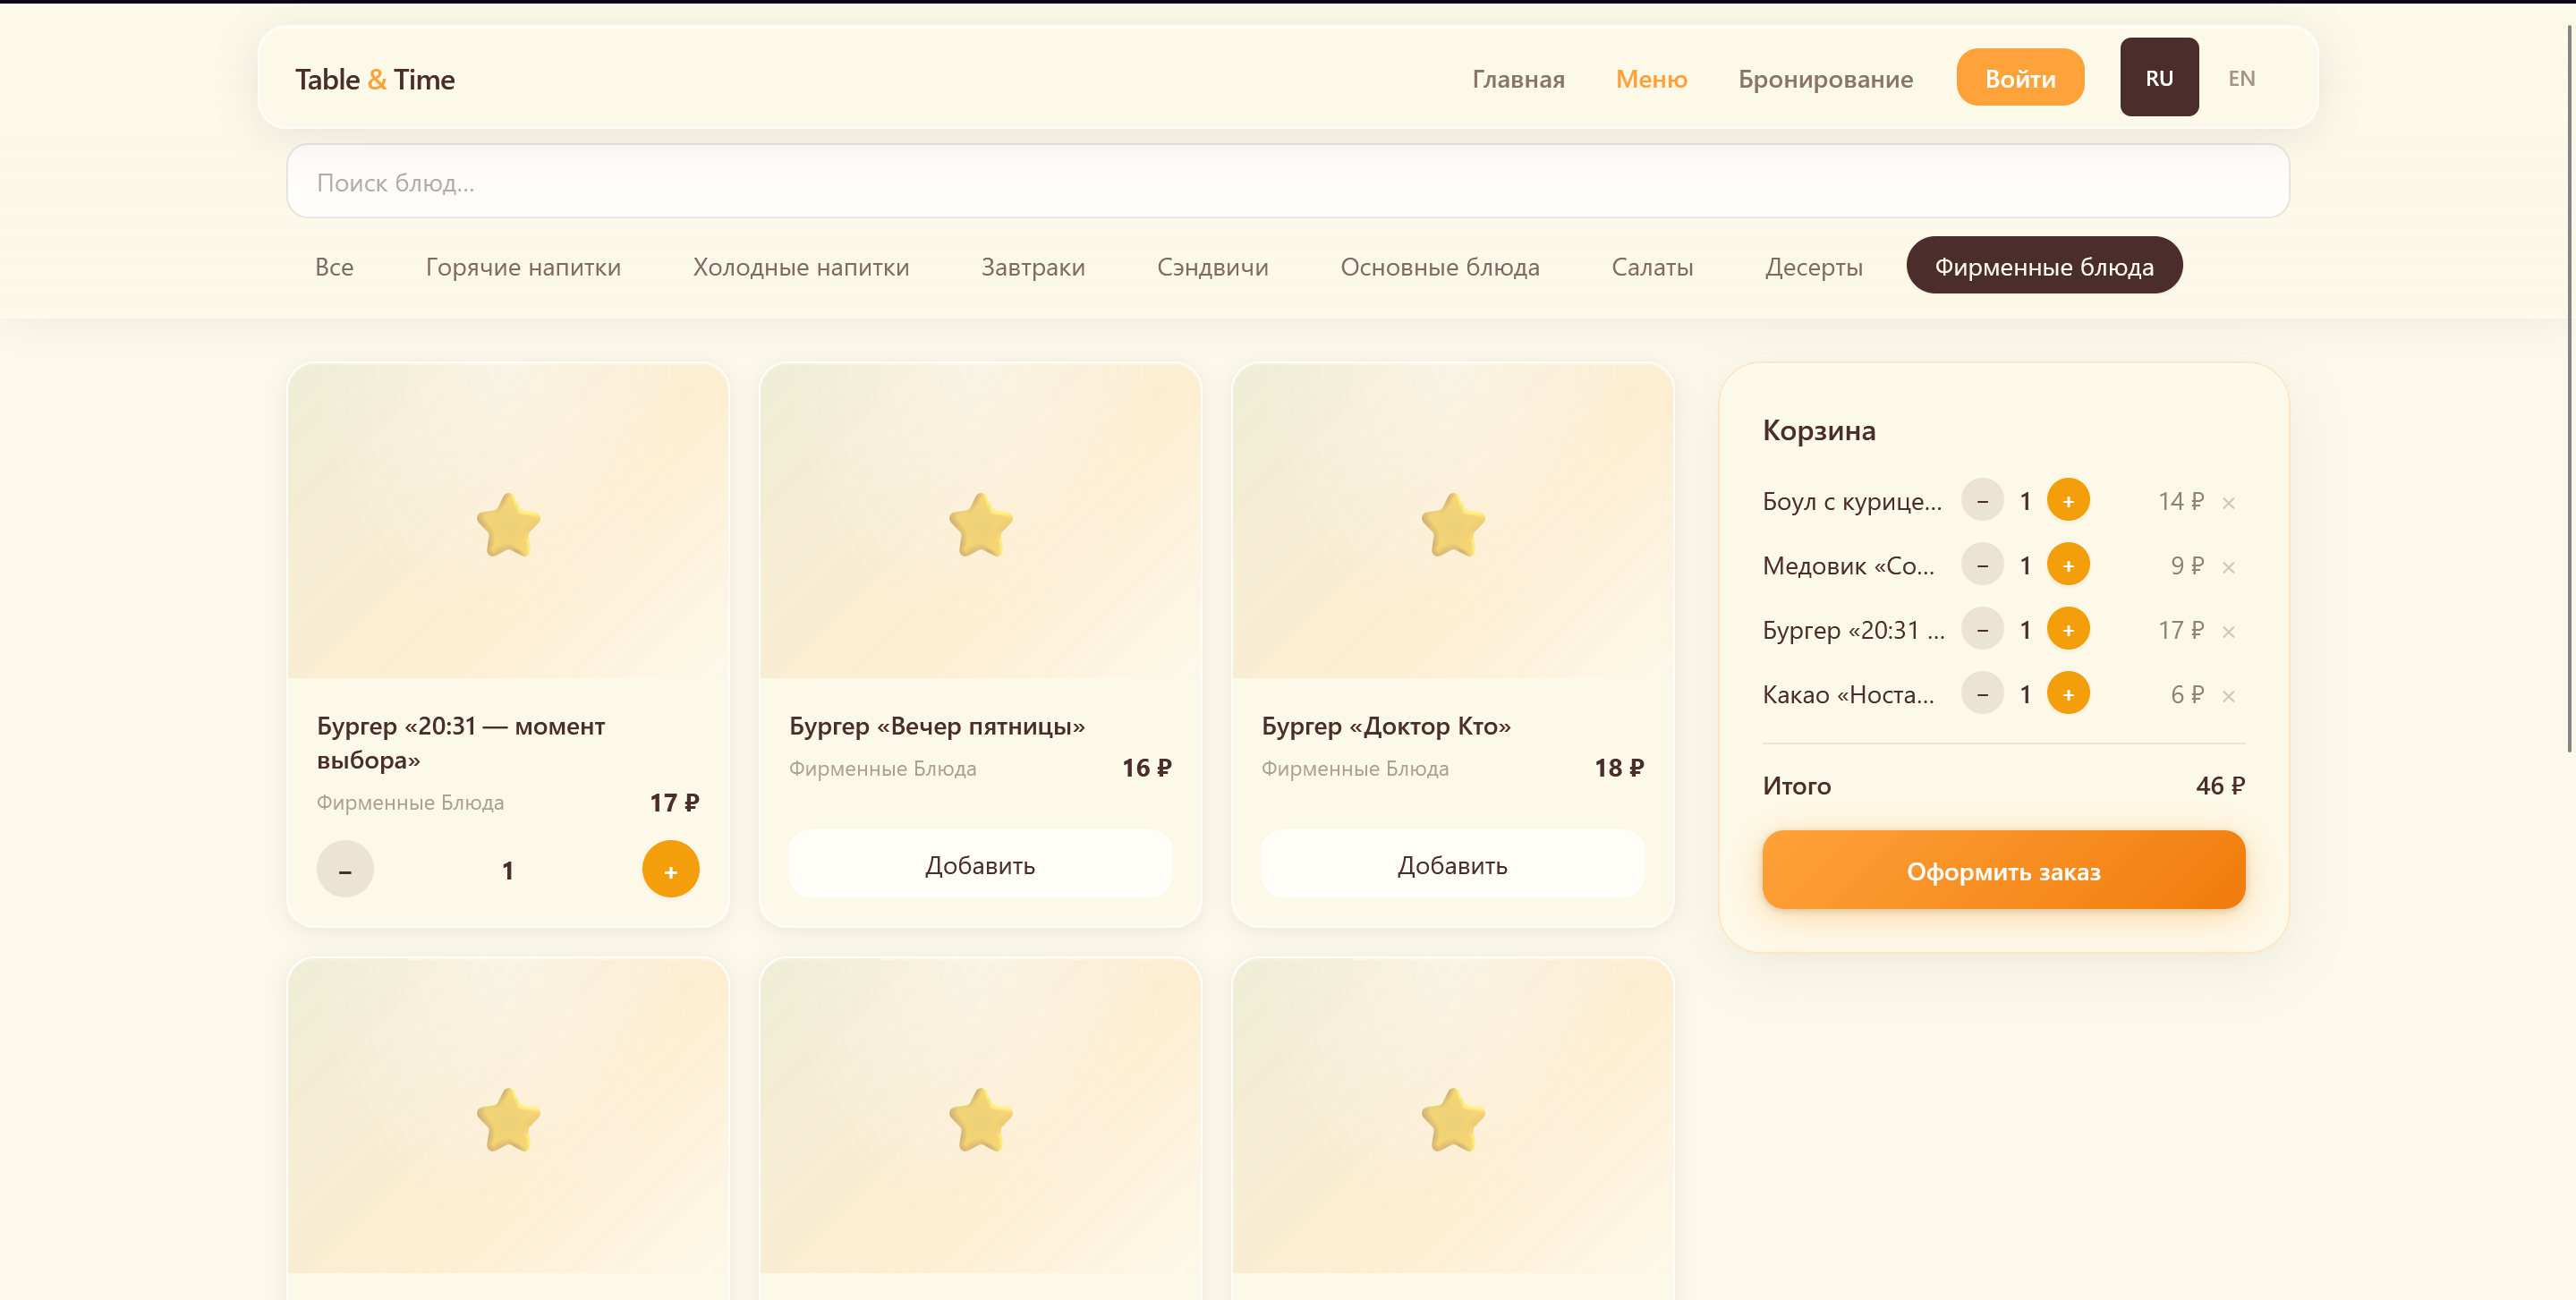
\includegraphics[width=0.85\textwidth]{images/menu.png}
\caption{Страница меню: панель категорий, сетка карточек блюд
         с изображениями и ценами}
\label{fig:menu}
\end{figure}

В приложении реализован переключатель языка интерфейса. При выборе
английской локали названия блюд отображаются на английском языке.
Для каждого блюда в базе данных хранятся оба варианта названия: на
русском (поле \texttt{name}) и на английском (поле \texttt{nameEn}).

Блюда, отключённые администратором, не отображаются посетителям,
однако остаются видимыми в панели администрирования
с соответствующей пометкой.

% ----------------------------------------------------------------
\subsection{Реализация страницы бронирования столов}
% ----------------------------------------------------------------

Страница бронирования отображает интерактивную карту зала
с расположением всех столов. Каждый стол обозначен цветным кружком,
цвет которого соответствует текущему статусу: зелёный~--- свободен,
жёлтый~--- забронирован, красный~--- занят, серый~--- убирается.
Все кружки сопровождаются анимацией пульсации, цвет которой
соответствует цвету статуса.

По умолчанию карта отображает актуальную ситуацию в зале на текущий
момент. При наведении на стол со статусом «убирается» отображается
всплывающая подсказка с обратным отсчётом времени до освобождения.

\begin{figure}[H]
\centering
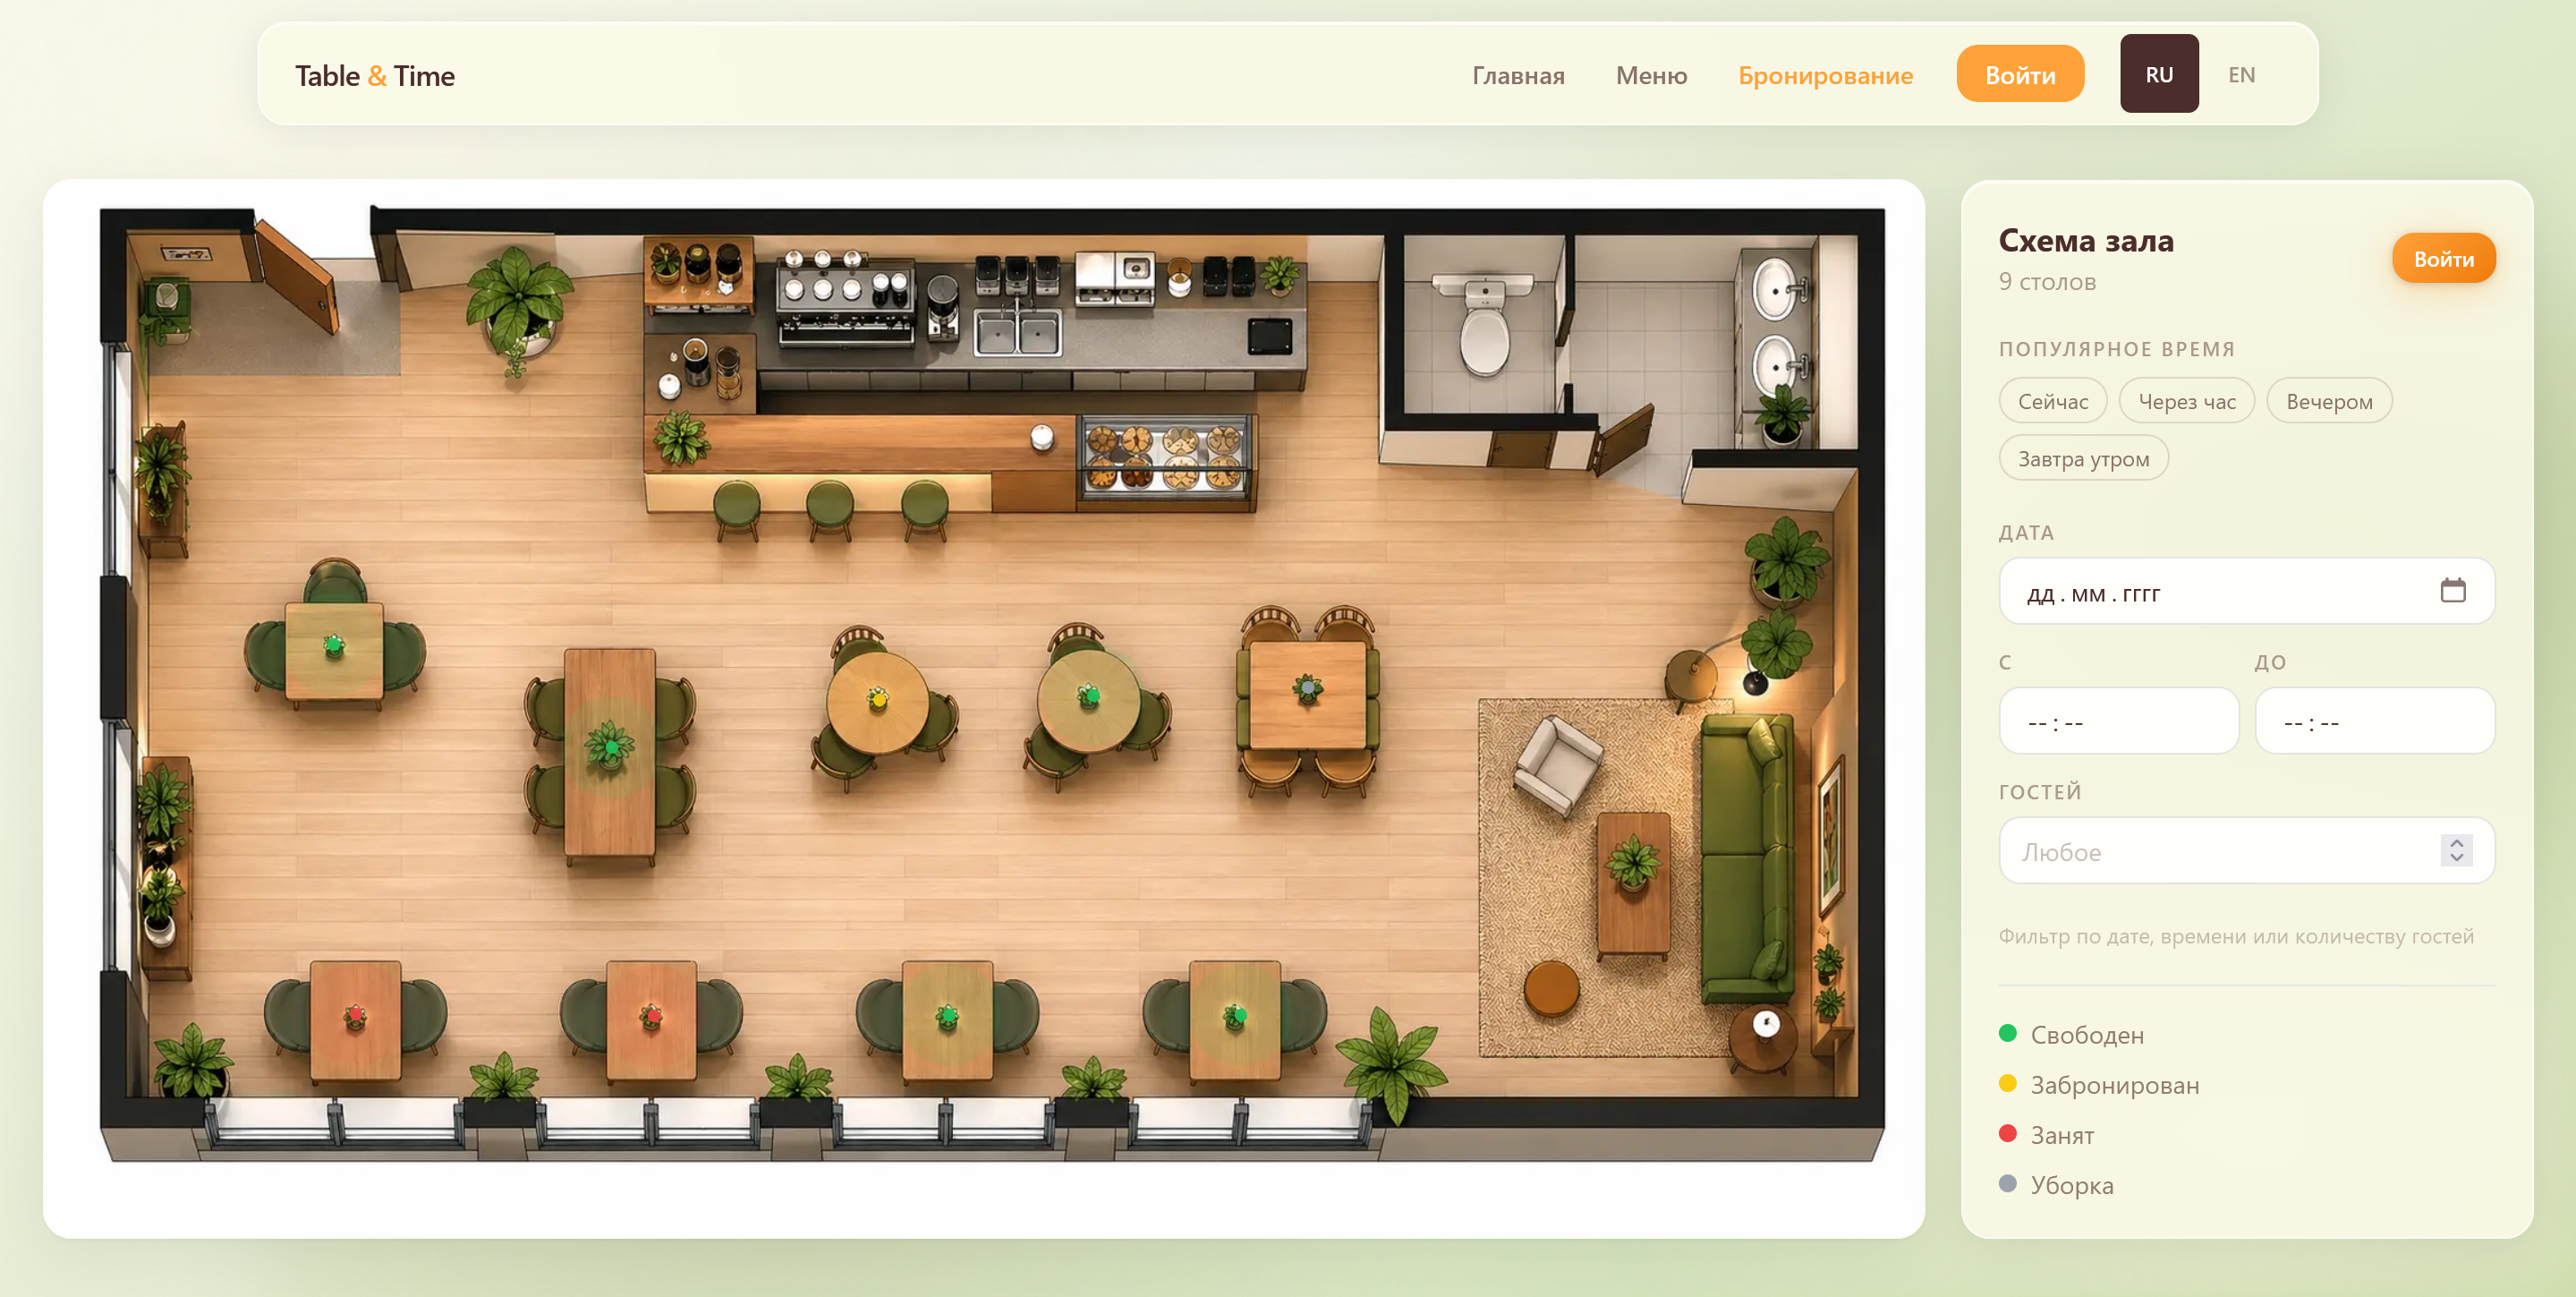
\includegraphics[width=0.85\textwidth]{images/tables1.png}
\caption{Карта столов в режиме просмотра без активного фильтра:
         столы отображают реальные статусы с цветовой индикацией}
\label{fig:tables_default}
\end{figure}

Для выбора стола под бронирование пользователь активирует панель
фильтра, где указывает дату, время начала и окончания визита,
а также количество гостей. После применения фильтра доступные для
бронирования столы подсвечиваются зелёным цветом, недоступные
сохраняют свой статусный цвет.

\begin{figure}[H]
\centering
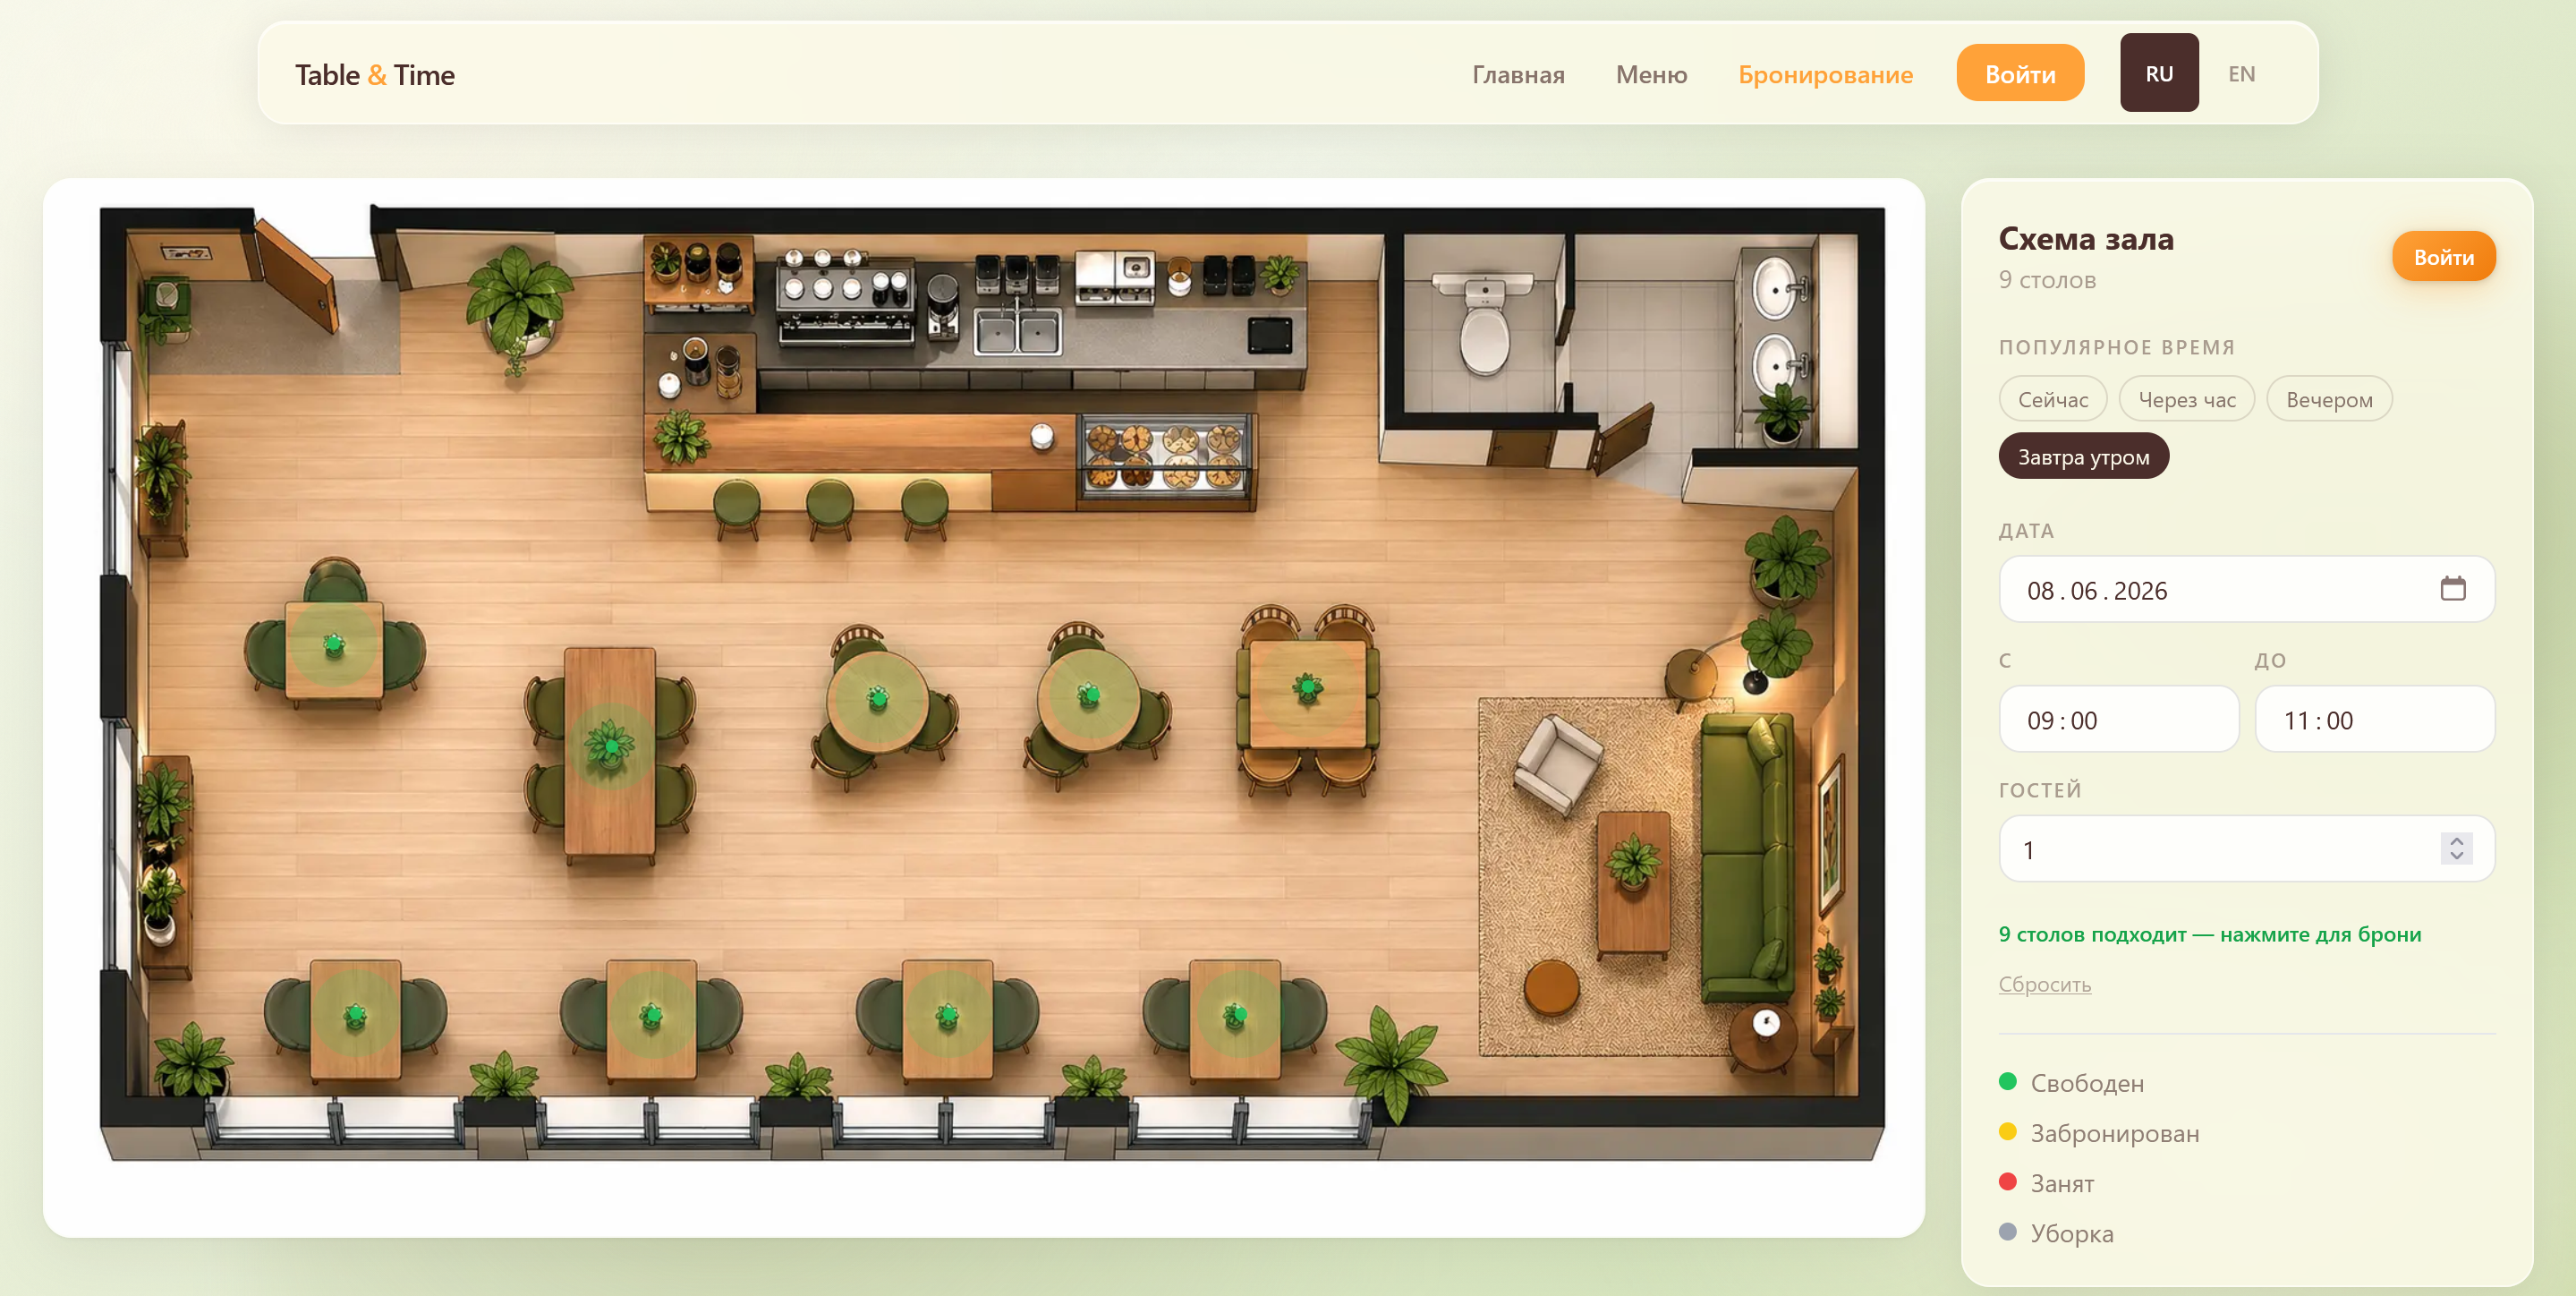
\includegraphics[width=0.85\textwidth]{images/tables2.png}
\caption{Карта столов с активным фильтром: доступные столы выделены
         зелёным, недоступные сохраняют цвет статуса}
\label{fig:tables_filter}
\end{figure}

Стол считается доступным для выбранного интервала, если не существует
пересекающегося подтверждённого бронирования. Столы в статусе
\texttt{OCCUPIED} допускают бронирование, если запрашиваемое время
начинается не ранее чем через два часа от текущего момента. Столы
в статусе \texttt{CLEANING} доступны для бронирования, если
к началу визита уборка заведомо завершится.

После выбора стола открывается форма подтверждения бронирования
с параметрами выбранного временного слота и вместимостью стола.

\begin{figure}[H]
\centering
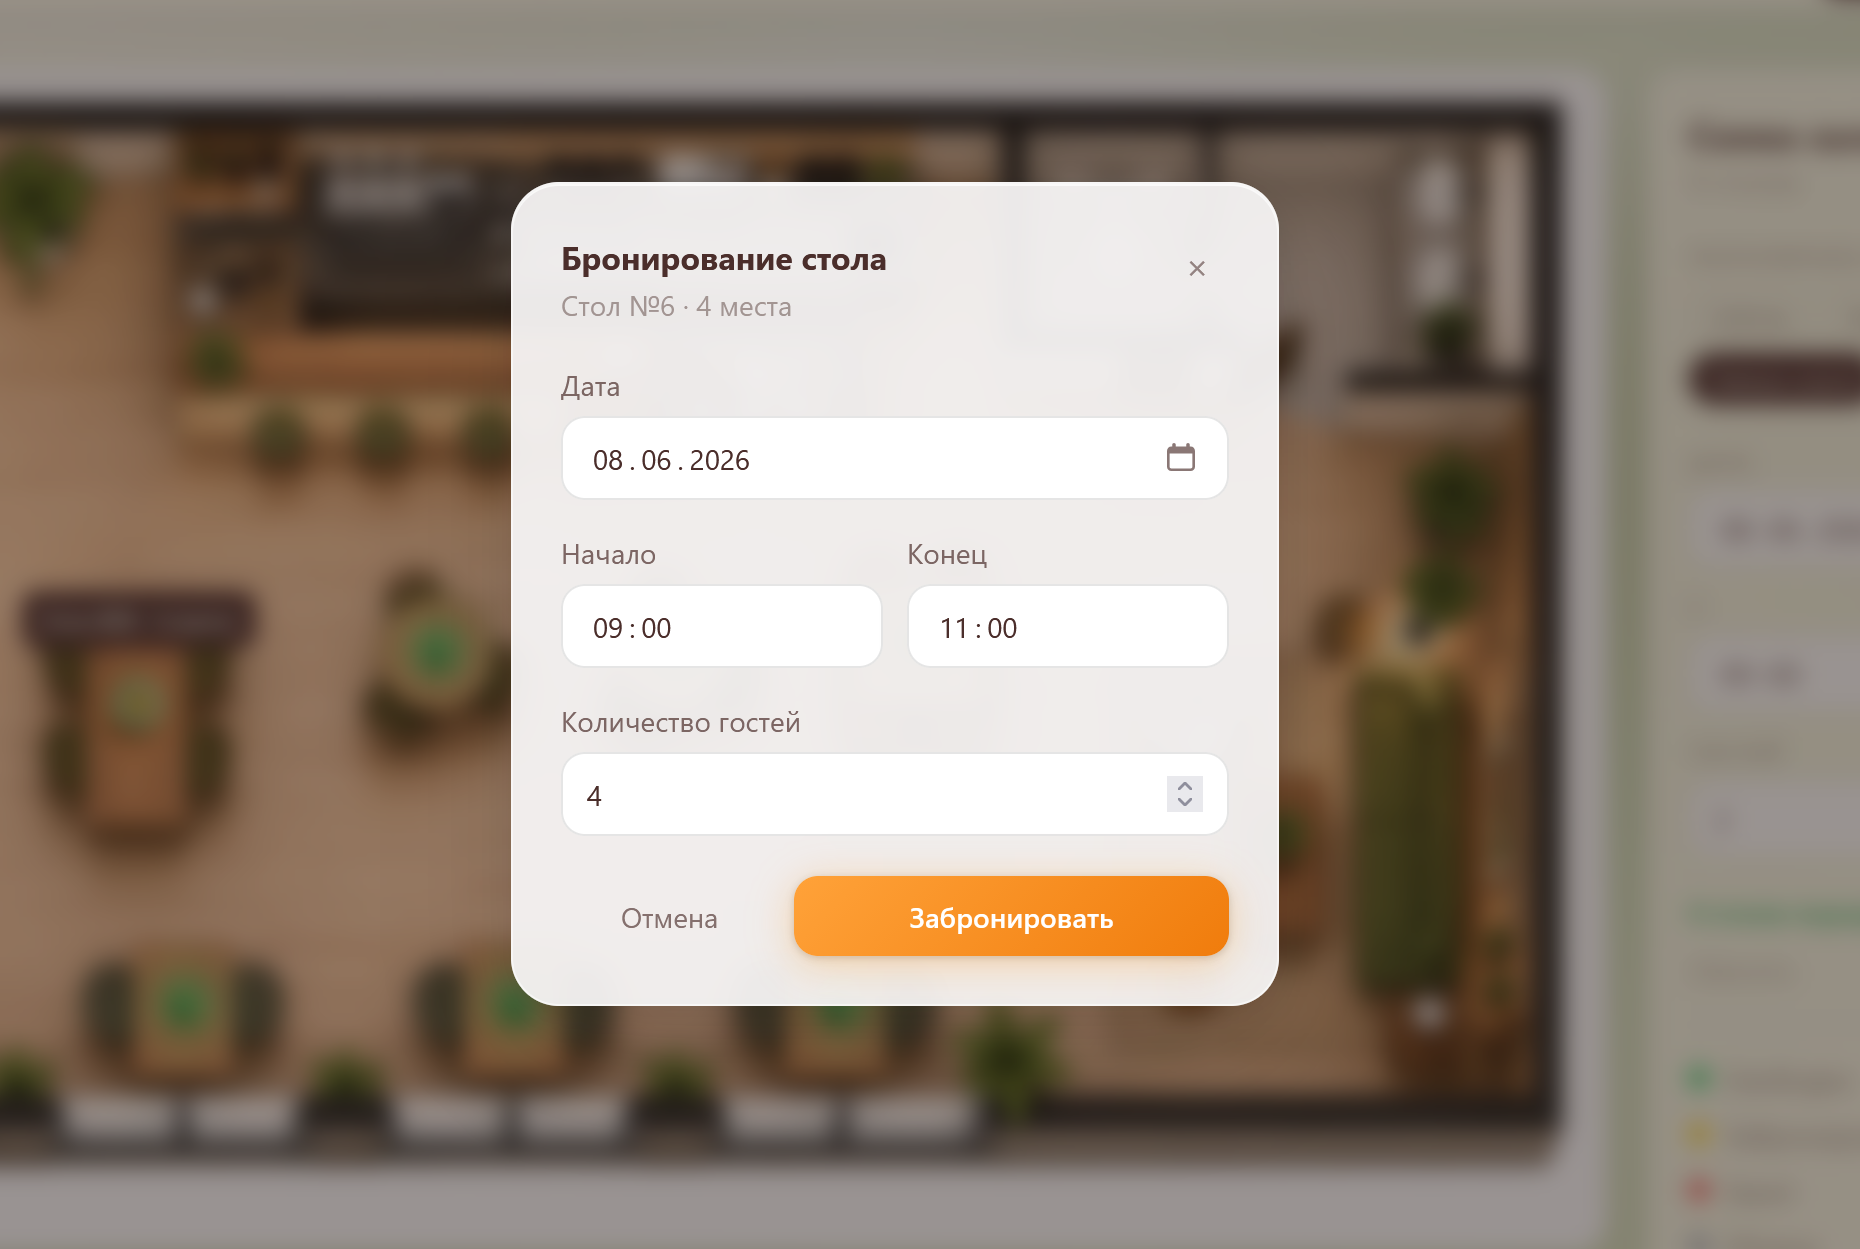
\includegraphics[width=0.85\textwidth]{images/tables_form.png}
\caption{Форма подтверждения бронирования: выбранный стол, дата,
         время, количество гостей, кнопка подтверждения}
\label{fig:booking_form}
\end{figure}

% ----------------------------------------------------------------
\subsection{Реализация системы статусов столов в реальном времени}
% ----------------------------------------------------------------

Статус каждого стола изменяется автоматически со временем без
вмешательства пользователя. Для хранения момента истечения текущего
статуса в схеме базы данных предусмотрено поле
\texttt{statusExpiresAt}.

На бэкенде реализованы три типа таймеров в памяти процесса:
\begin{itemize}
  \item таймер уборки (\texttt{cleaningTimers}): по истечении
        10~минут стол автоматически переходит из статуса
        \texttt{CLEANING} в \texttt{FREE};
  \item таймер занятости (\texttt{occupiedTimers}): по истечении
        двух часов статус \texttt{OCCUPIED} снимается и состояние
        стола пересчитывается;
  \item таймер бронирования (\texttt{reservedTimers}): при
        наступлении времени начала бронирования стол переходит
        из \texttt{RESERVED} в \texttt{OCCUPIED}.
\end{itemize}

При запуске сервера метод \texttt{onModuleInit} восстанавливает все
активные таймеры из базы данных, вычисляя оставшееся время до
истечения каждого статуса.

На фронтенде статусы отображаются в реальном времени с помощью хука
\texttt{useNow()}, обновляющего текущее время каждую секунду.
Функция \texttt{getEffectiveStatus()} сравнивает текущее время
с полем \texttt{statusExpiresAt} и возвращает \texttt{FREE}, если
срок действия статуса истёк, даже если сервер ещё не обновил запись
в базе данных. 

% ----------------------------------------------------------------
\subsection{Реализация оформления заказов}
% ----------------------------------------------------------------

В приложении поддерживаются три типа заказов:
\begin{itemize}
  \item \texttt{DINE\_IN}~--- заказ в зале с привязкой к конкретному
        столу;
  \item \texttt{DELIVERY}~--- доставка по указанному адресу;
  \item \texttt{TAKEAWAY}~--- заказ навынос.
\end{itemize}

Форма оформления заказа включает выбор позиций из меню и указание
типа заказа. Для доставки дополнительно вводится адрес, для заказа
в зале~--- номер стола. Предусмотрена возможность оформить заказ
заранее, указав желаемое время подачи.

\begin{figure}[H]
\centering
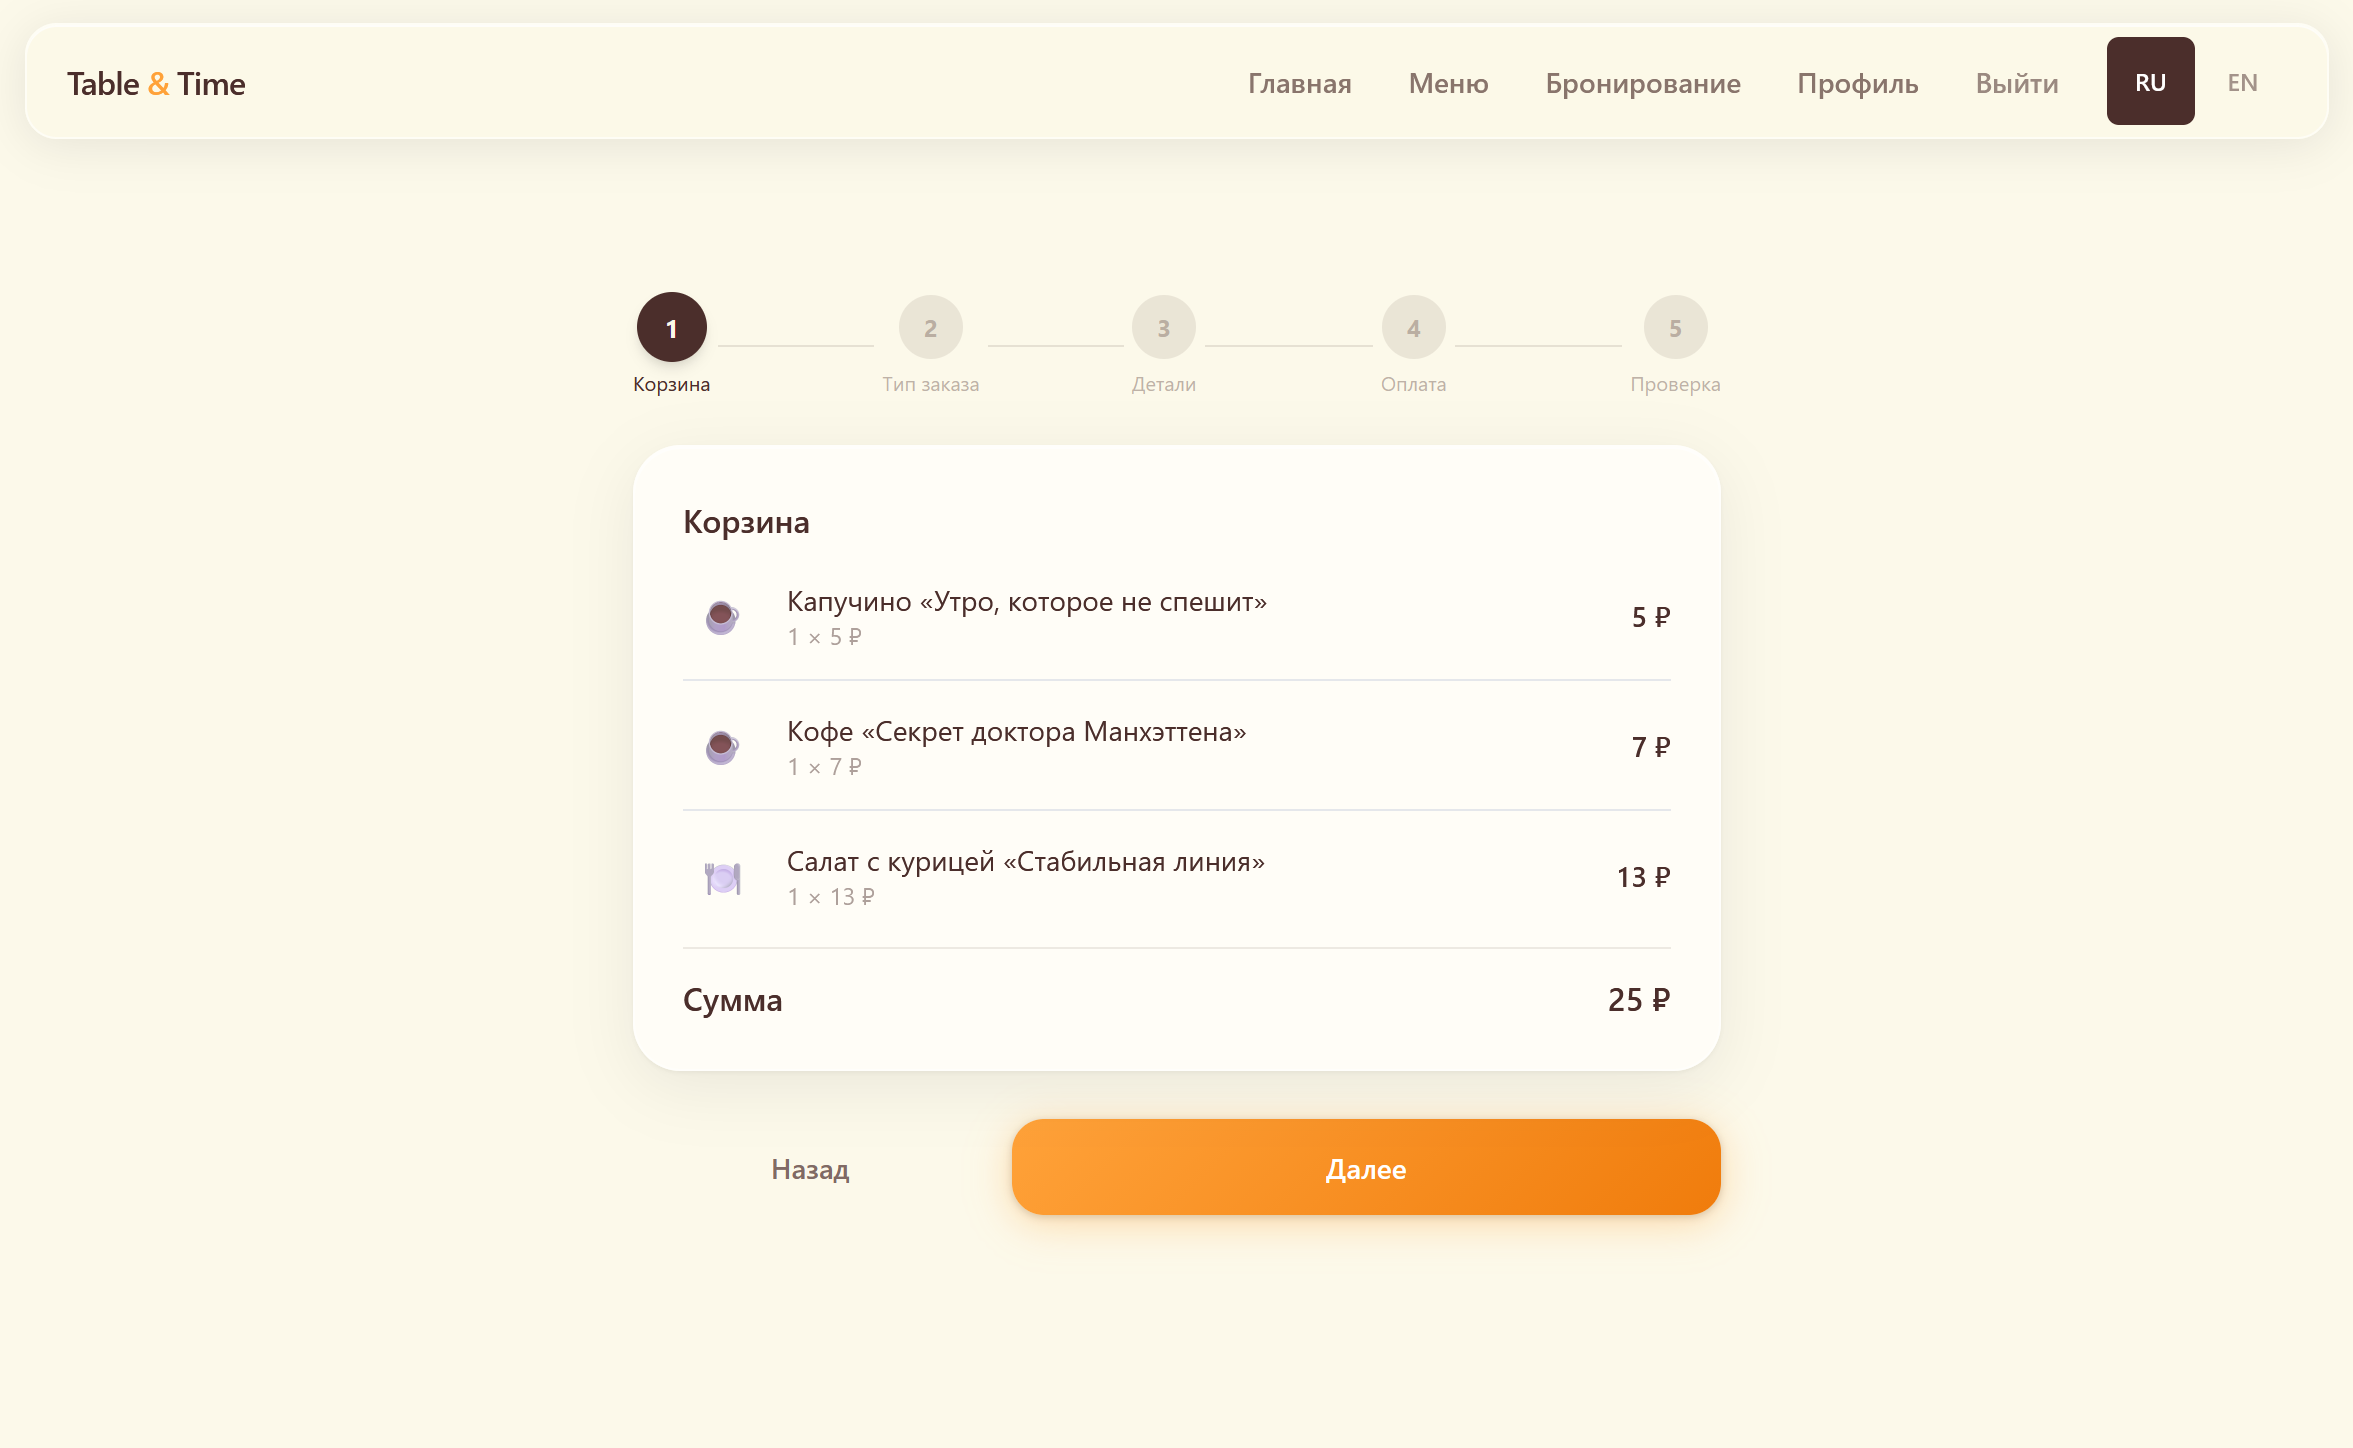
\includegraphics[width=0.85\textwidth]{images/order_form.png}
\caption{Форма оформления заказа: выбор блюд, тип заказа,
         поле адреса или стола}
\label{fig:order_form}
\end{figure}

Жизненный цикл заказа реализован в виде конечного автомата:
\texttt{CREATED} $\to$ \texttt{CONFIRMED} $\to$ \texttt{PREPARING}
$\to$ \texttt{READY} $\to$ \texttt{COMPLETED}. Также предусмотрен
статус \texttt{CANCELLED} для отменённых заказов. Управление
статусами осуществляется официантом и администратором: для каждого
этапа отображается кнопка перехода к следующему со понятной
подписью («Подтвердить», «Начать готовку», «Готово» и~т.\,д.).

% ----------------------------------------------------------------
\subsection{Реализация личного кабинета пользователя}
% ----------------------------------------------------------------

Личный кабинет предоставляет пользователю сводную информацию о его
активности. Страница разделена на две колонки: в левой расположена
сводная панель и блок управления, в правой~--- списки бронирований
и заказов.

В верхней части страницы отображается информационная панель
с четырьмя показателями: количество предстоящих бронирований,
количество активных заказов, общее число бронирований и общее число
заказов.

\begin{figure}[H]
\centering
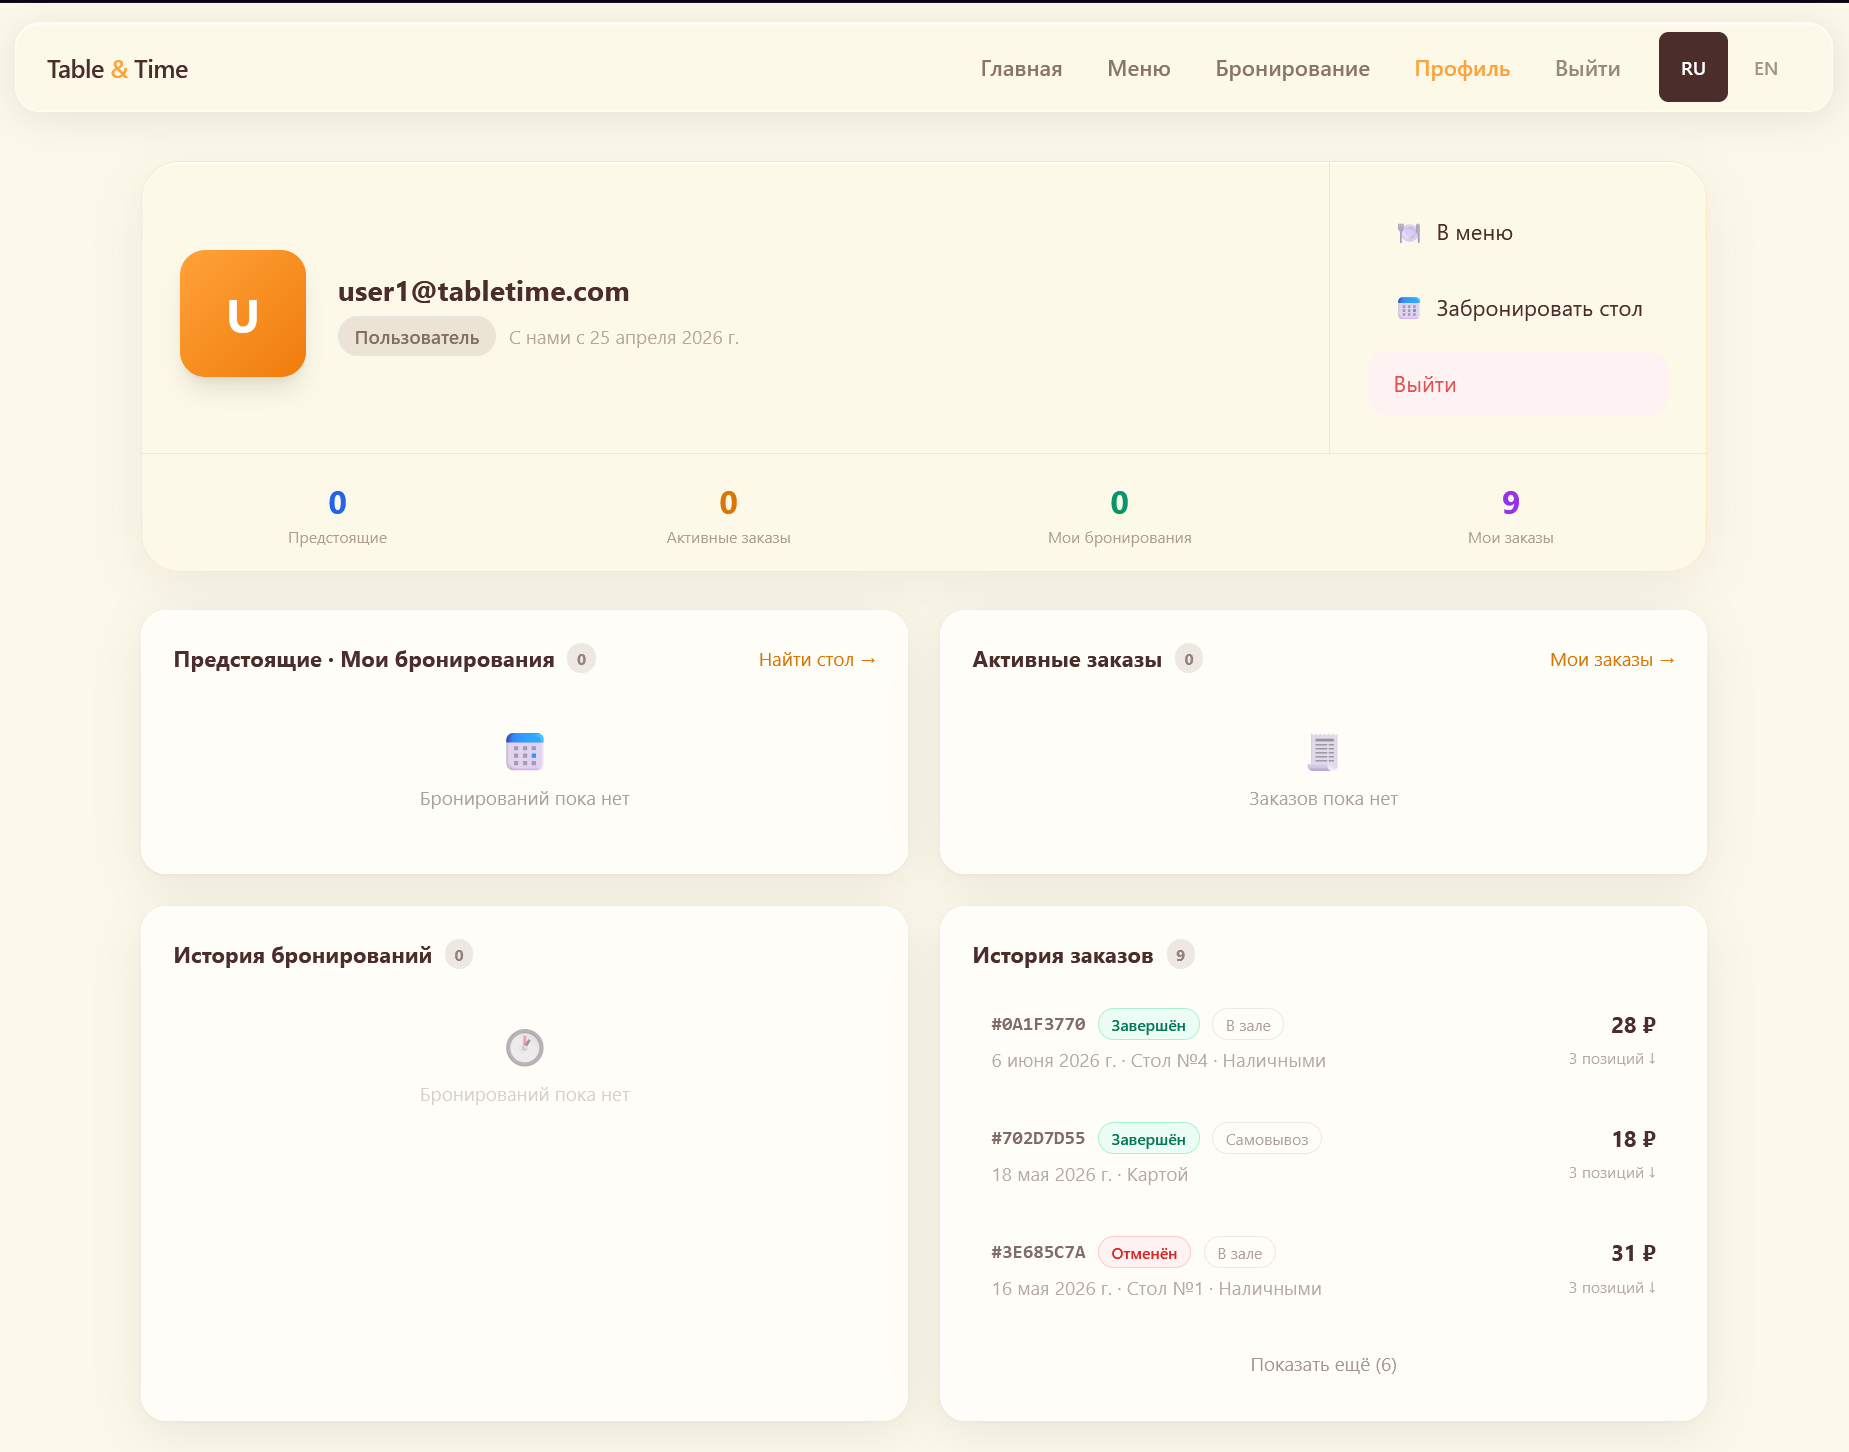
\includegraphics[width=0.85\textwidth]{images/profile.png}
\caption{Личный кабинет пользователя: панель со статистикой,
         список бронирований, список заказов}
\label{fig:profile}
\end{figure}

В разделе бронирований отображаются предстоящие и прошедшие записи
с указанием номера стола, даты, времени и количества гостей.
Пользователь может отменить предстоящее бронирование
непосредственно из личного кабинета. В разделе заказов отображается
история с указанием типа, состава, суммы и текущего статуса каждого
заказа.

% ----------------------------------------------------------------
\subsection{Реализация административной панели}
% ----------------------------------------------------------------

Административная панель доступна только пользователям с ролью
\texttt{ADMIN}. Панель организована в виде шести вкладок, каждая
из которых отвечает за отдельный раздел управления заведением.

\subsubsection{Вкладка «Аналитика»}

Вкладка аналитики отображает ключевые показатели работы заведения:
общую выручку, количество заказов, количество бронирований и
численность персонала. Данные формируются по всем записям в базе
данных и обновляются при каждом открытии вкладки.

\begin{figure}[H]
\centering
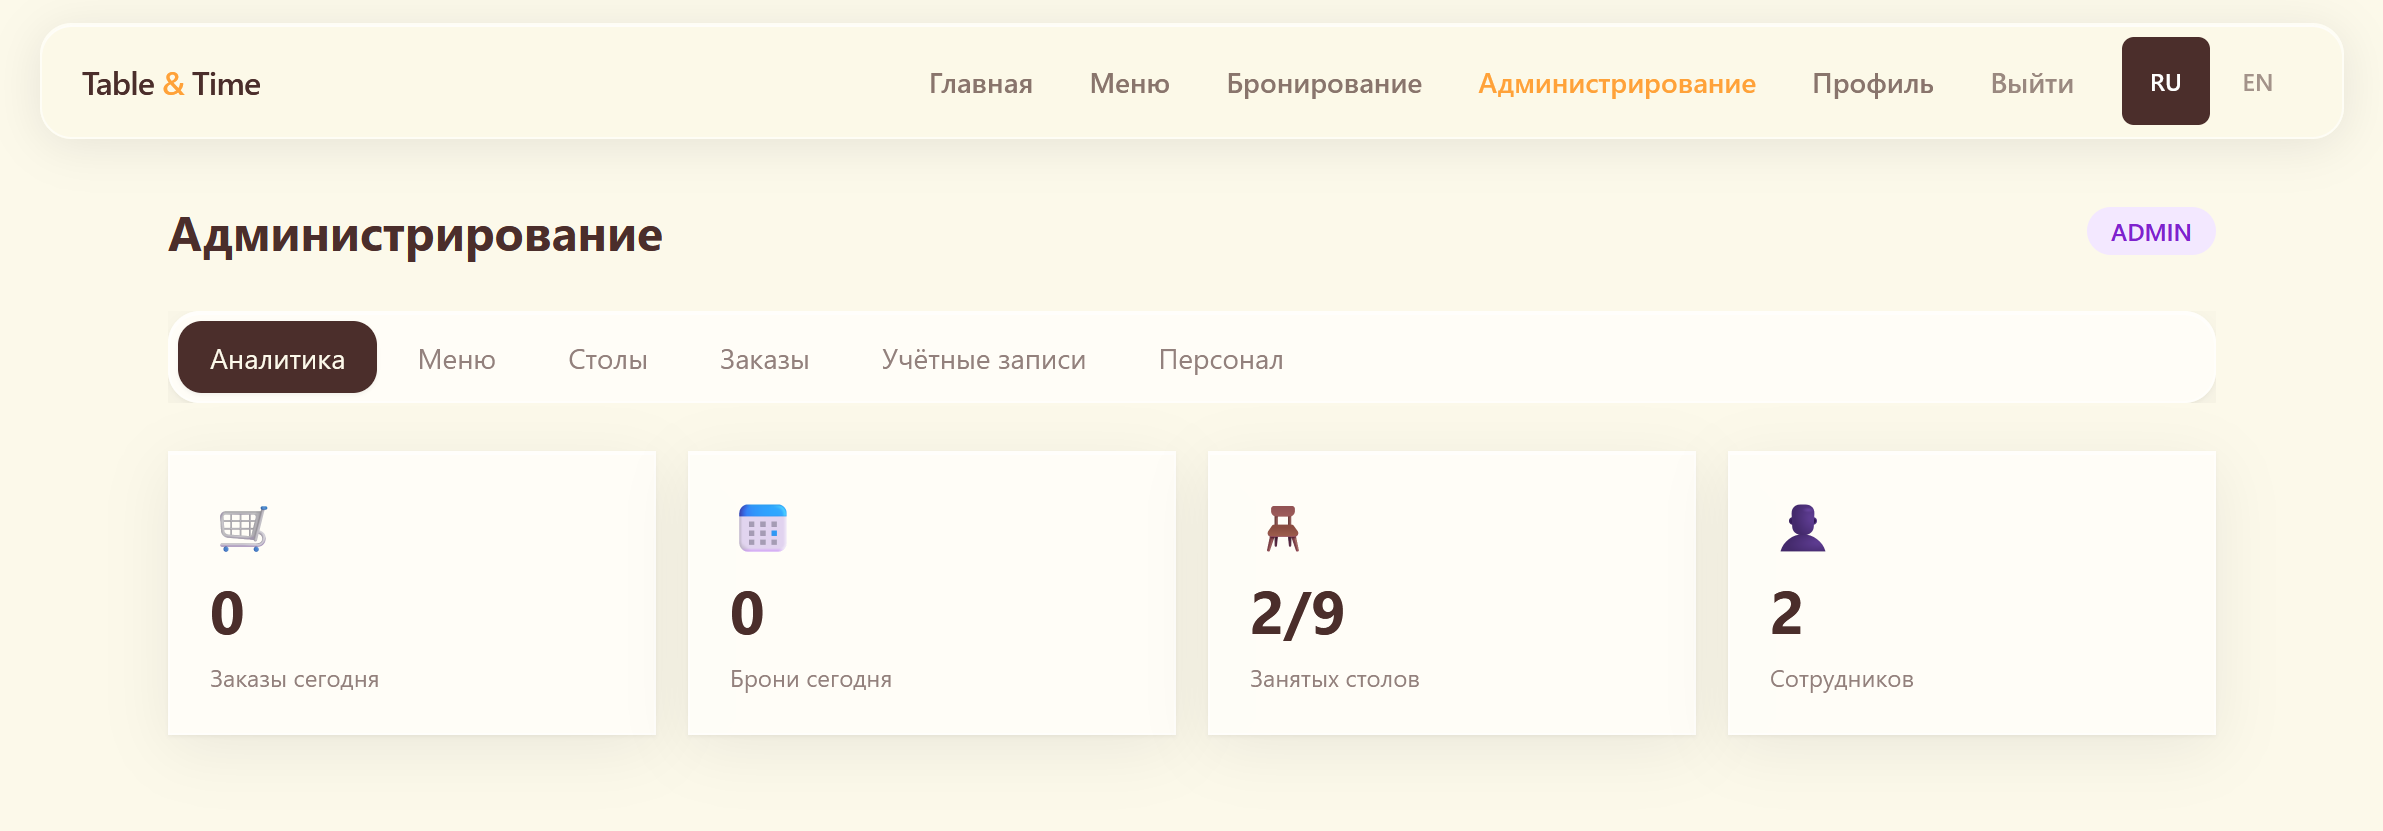
\includegraphics[width=0.85\textwidth]{images/analisys.png}
\caption{Вкладка «Аналитика»: четыре карточки с показателями}
\label{fig:admin_analytics}
\end{figure}

\subsubsection{Вкладка «Меню»}

Вкладка управления меню позволяет администратору добавлять,
редактировать и удалять блюда. Для каждого блюда задаются название
на русском и английском языках, цена, категория, изображение и
признак доступности. Недоступные блюда скрыты от посетителей,
однако сохраняются в базе данных и могут быть повторно активированы.

\begin{figure}[H]
\centering
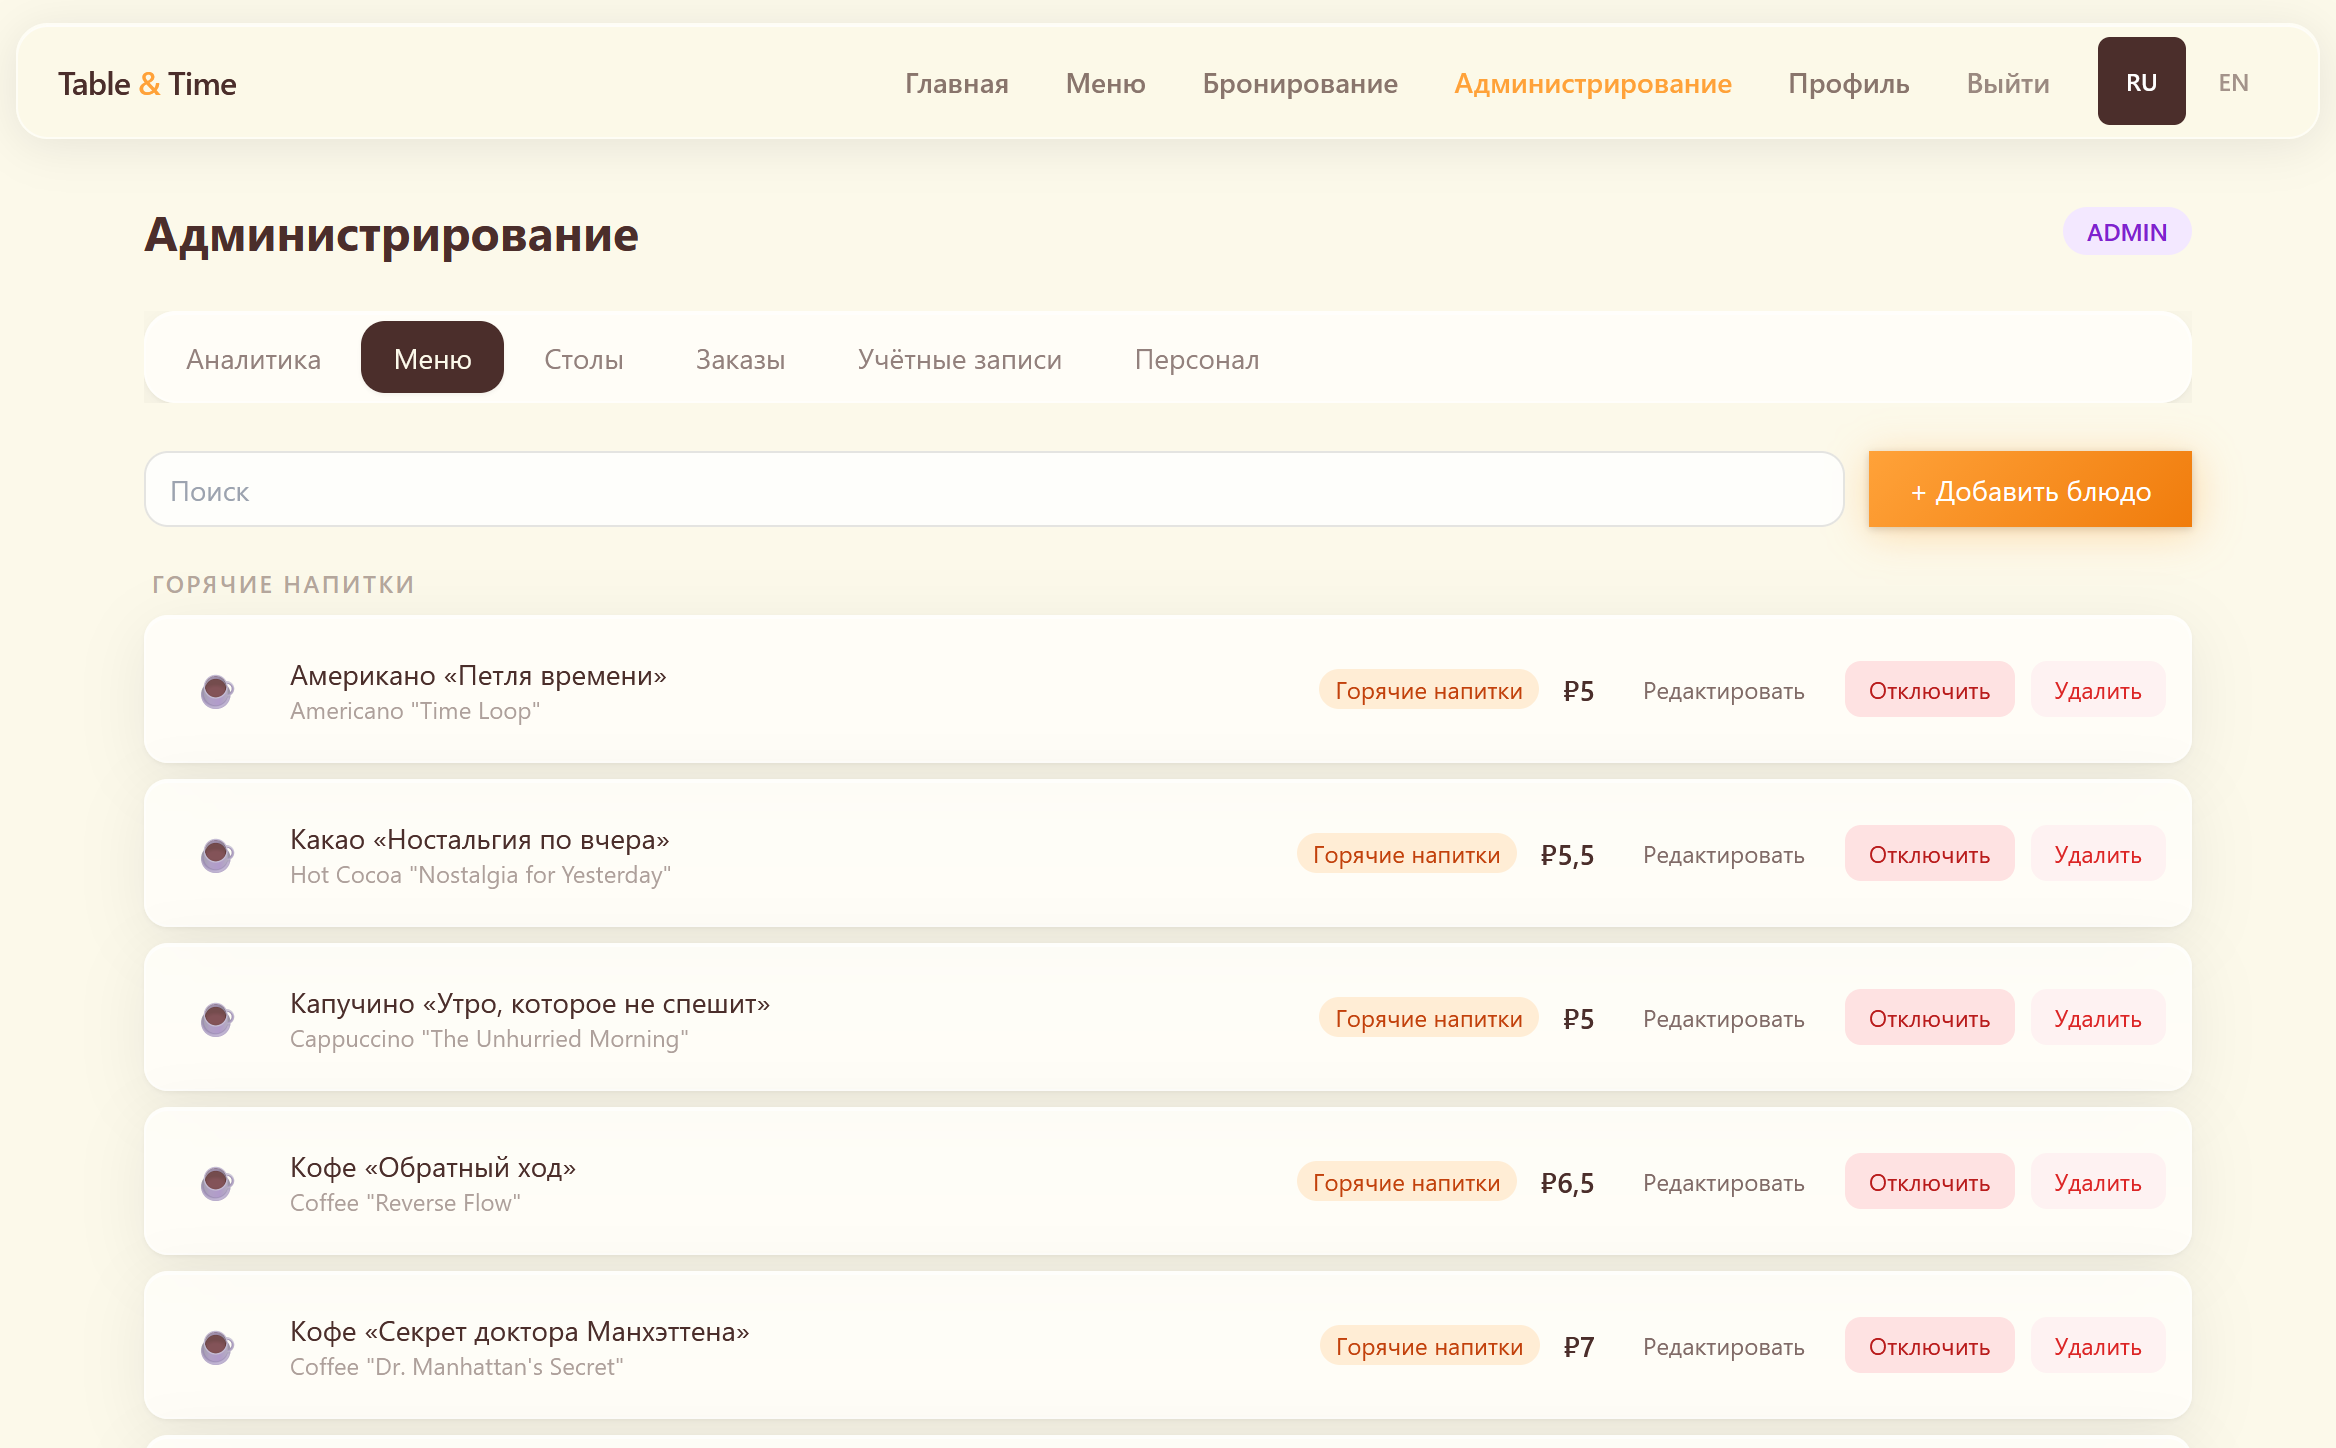
\includegraphics[width=0.85\textwidth]{images/adm_menu.png}
\caption{Вкладка «Меню»: список блюд по категориям и форма
         добавления/редактирования блюда}
\label{fig:admin_menu}
\end{figure}

\subsubsection{Вкладка «Столы»}

Вкладка управления столами отображает карточки всех столов,
окрашенные в цвет текущего статуса: зелёный~--- свободен,
жёлтый~--- забронирован, красный~--- занят, серый~--- убирается.
В верхней части вкладки расположена легенда, показывающая количество
столов в каждом из четырёх статусов.

Для каждого стола администратор может изменить статус вручную,
назначить или снять официанта, а также отредактировать параметры
(вместимость, расположение на карте).

\begin{figure}[H]
\centering
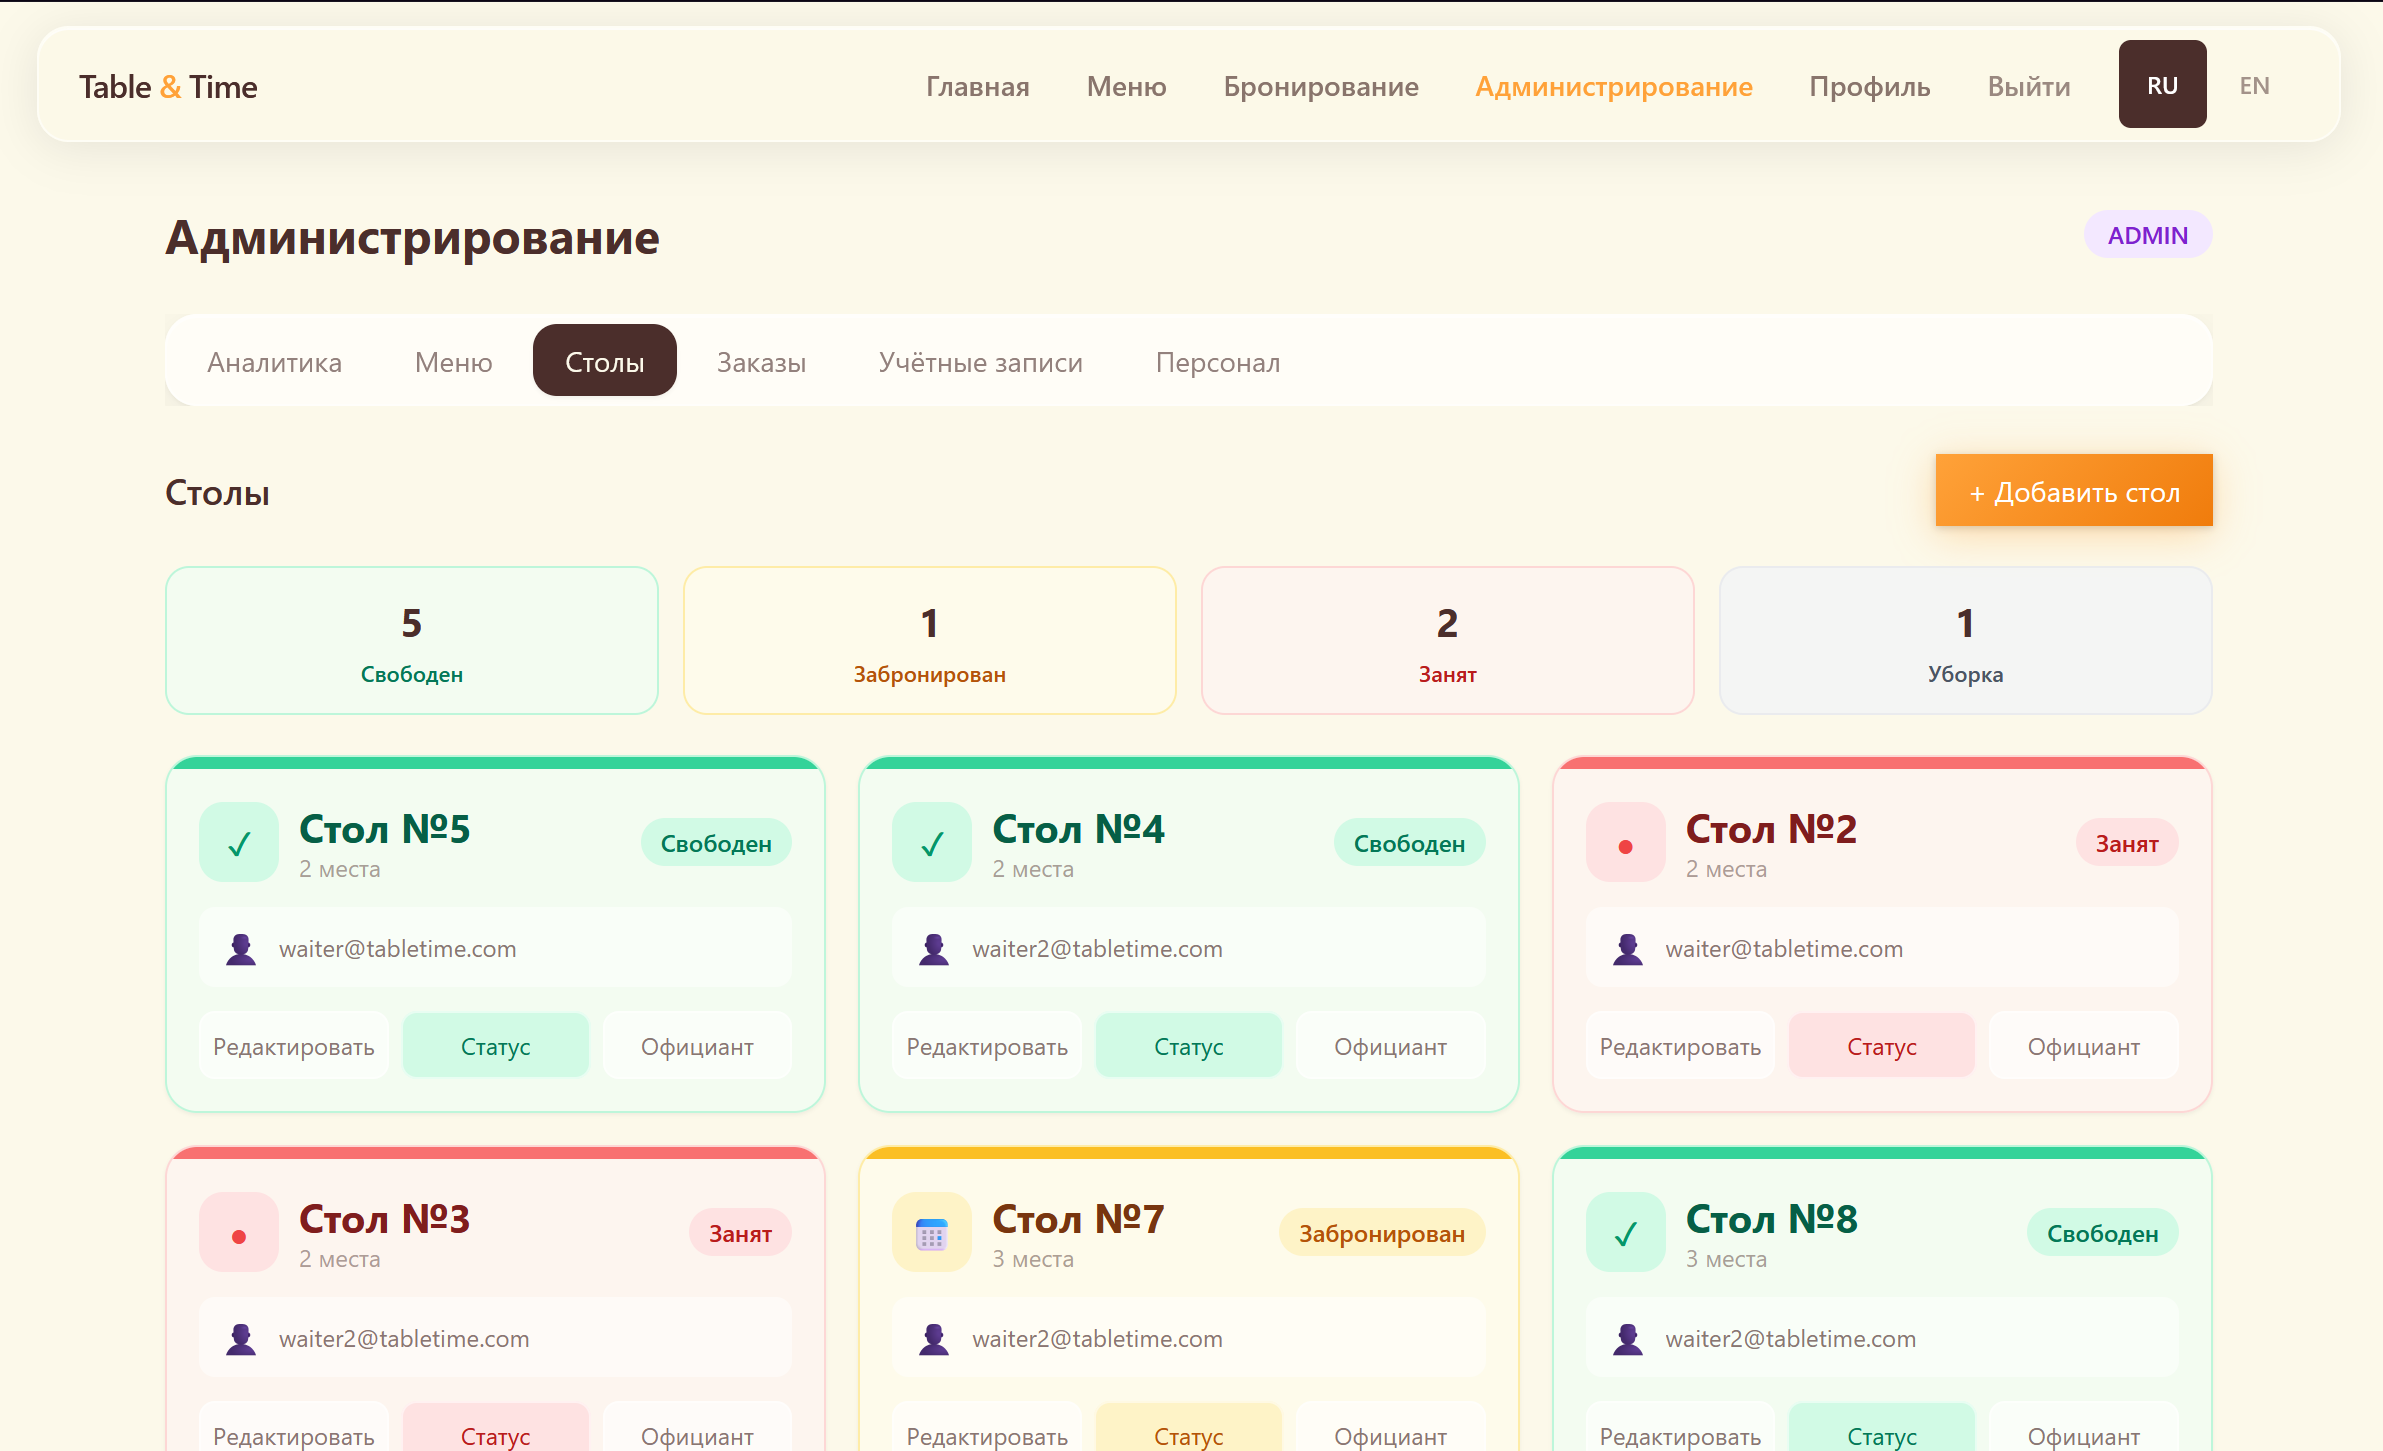
\includegraphics[width=0.85\textwidth]{images/adm_tables.png}
\caption{Вкладка «Столы»: легенда статусов с количеством,
         цветные карточки столов с кнопками управления}
\label{fig:admin_tables}
\end{figure}

\subsubsection{Вкладка «Заказы»}

Вкладка заказов предназначена для управления текущими заказами.
Отображаются все активные заказы с указанием типа, состава, суммы
и текущего статуса. Для каждого заказа доступна кнопка перехода
к следующему статусу в соответствии с автоматом состояний.

\begin{figure}[H]
\centering
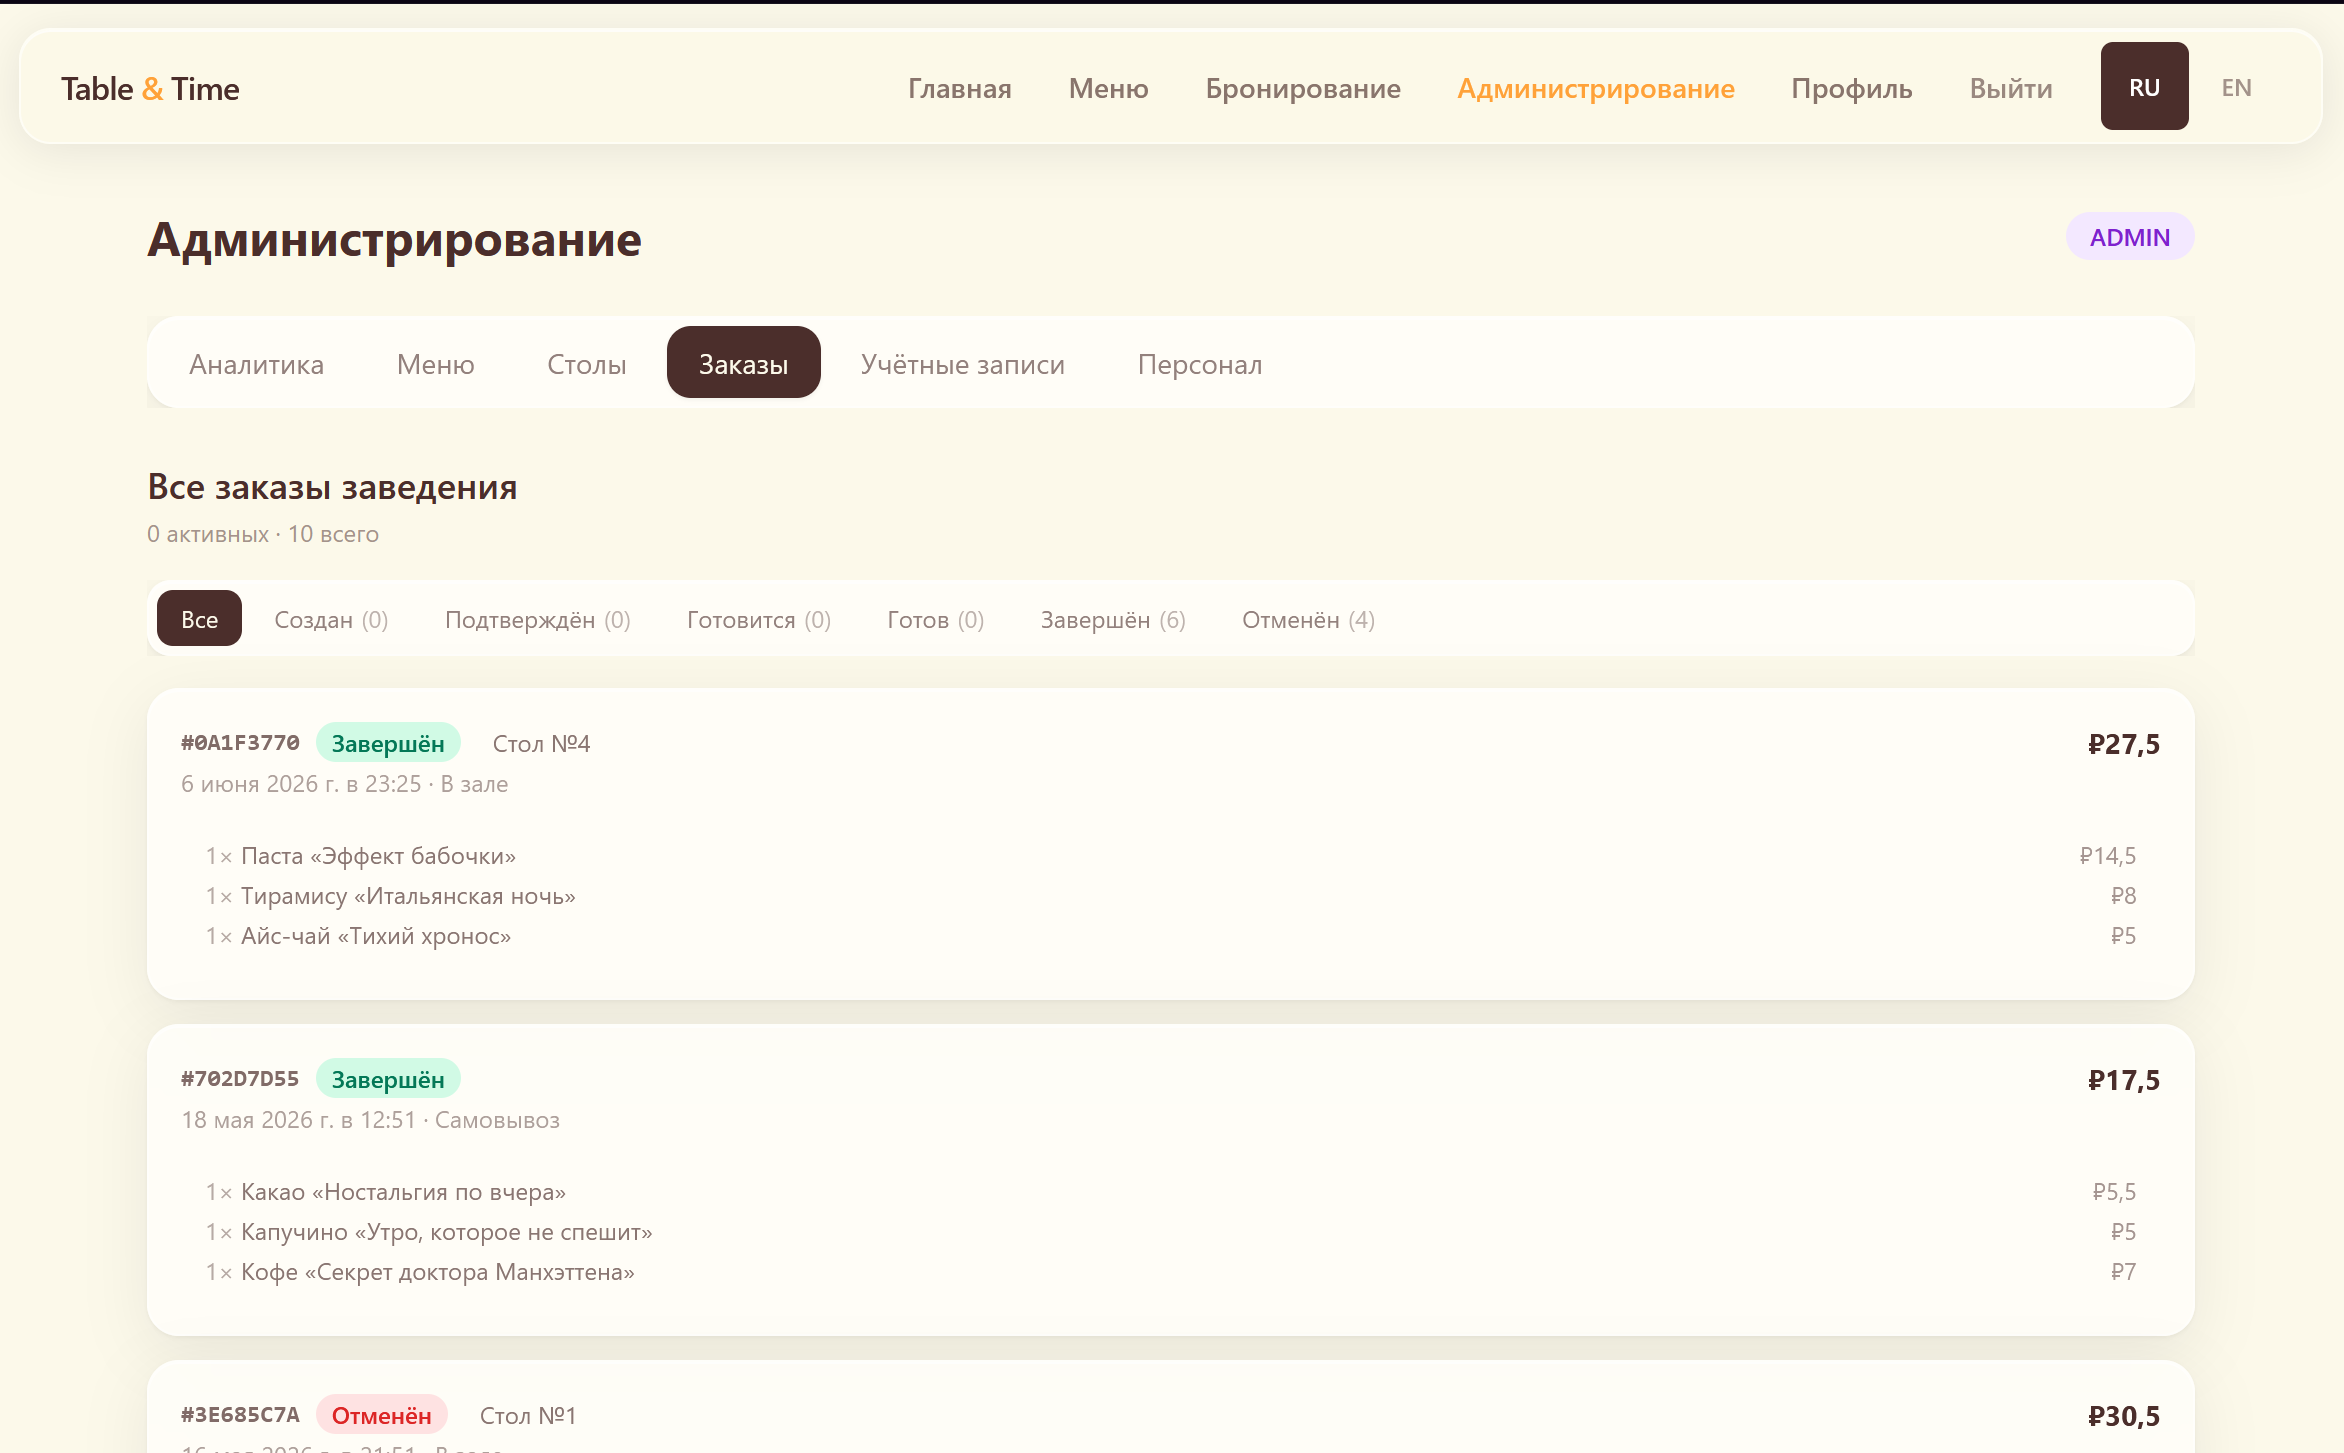
\includegraphics[width=0.85\textwidth]{images/orders.png}
\caption{Вкладка «Заказы»: список заказов с составом, суммой,
         статусом и кнопками управления}
\label{fig:admin_orders}
\end{figure}

\subsubsection{Вкладка «Учетные записи»}

Вкладка аккаунтов позволяет администратору просматривать список всех
зарегистрированных пользователей с фильтрацией по роли и поиском по
электронной почте. Для каждого пользователя доступно изменение роли
(\texttt{USER} или \texttt{WAITER}) и удаление аккаунта. Реализована
форма создания нового аккаунта с указанием электронной почты, пароля
и роли. Пароль должен содержать не менее восьми символов, включая
заглавную букву, строчную букву и цифру.

\begin{figure}[H]
\centering
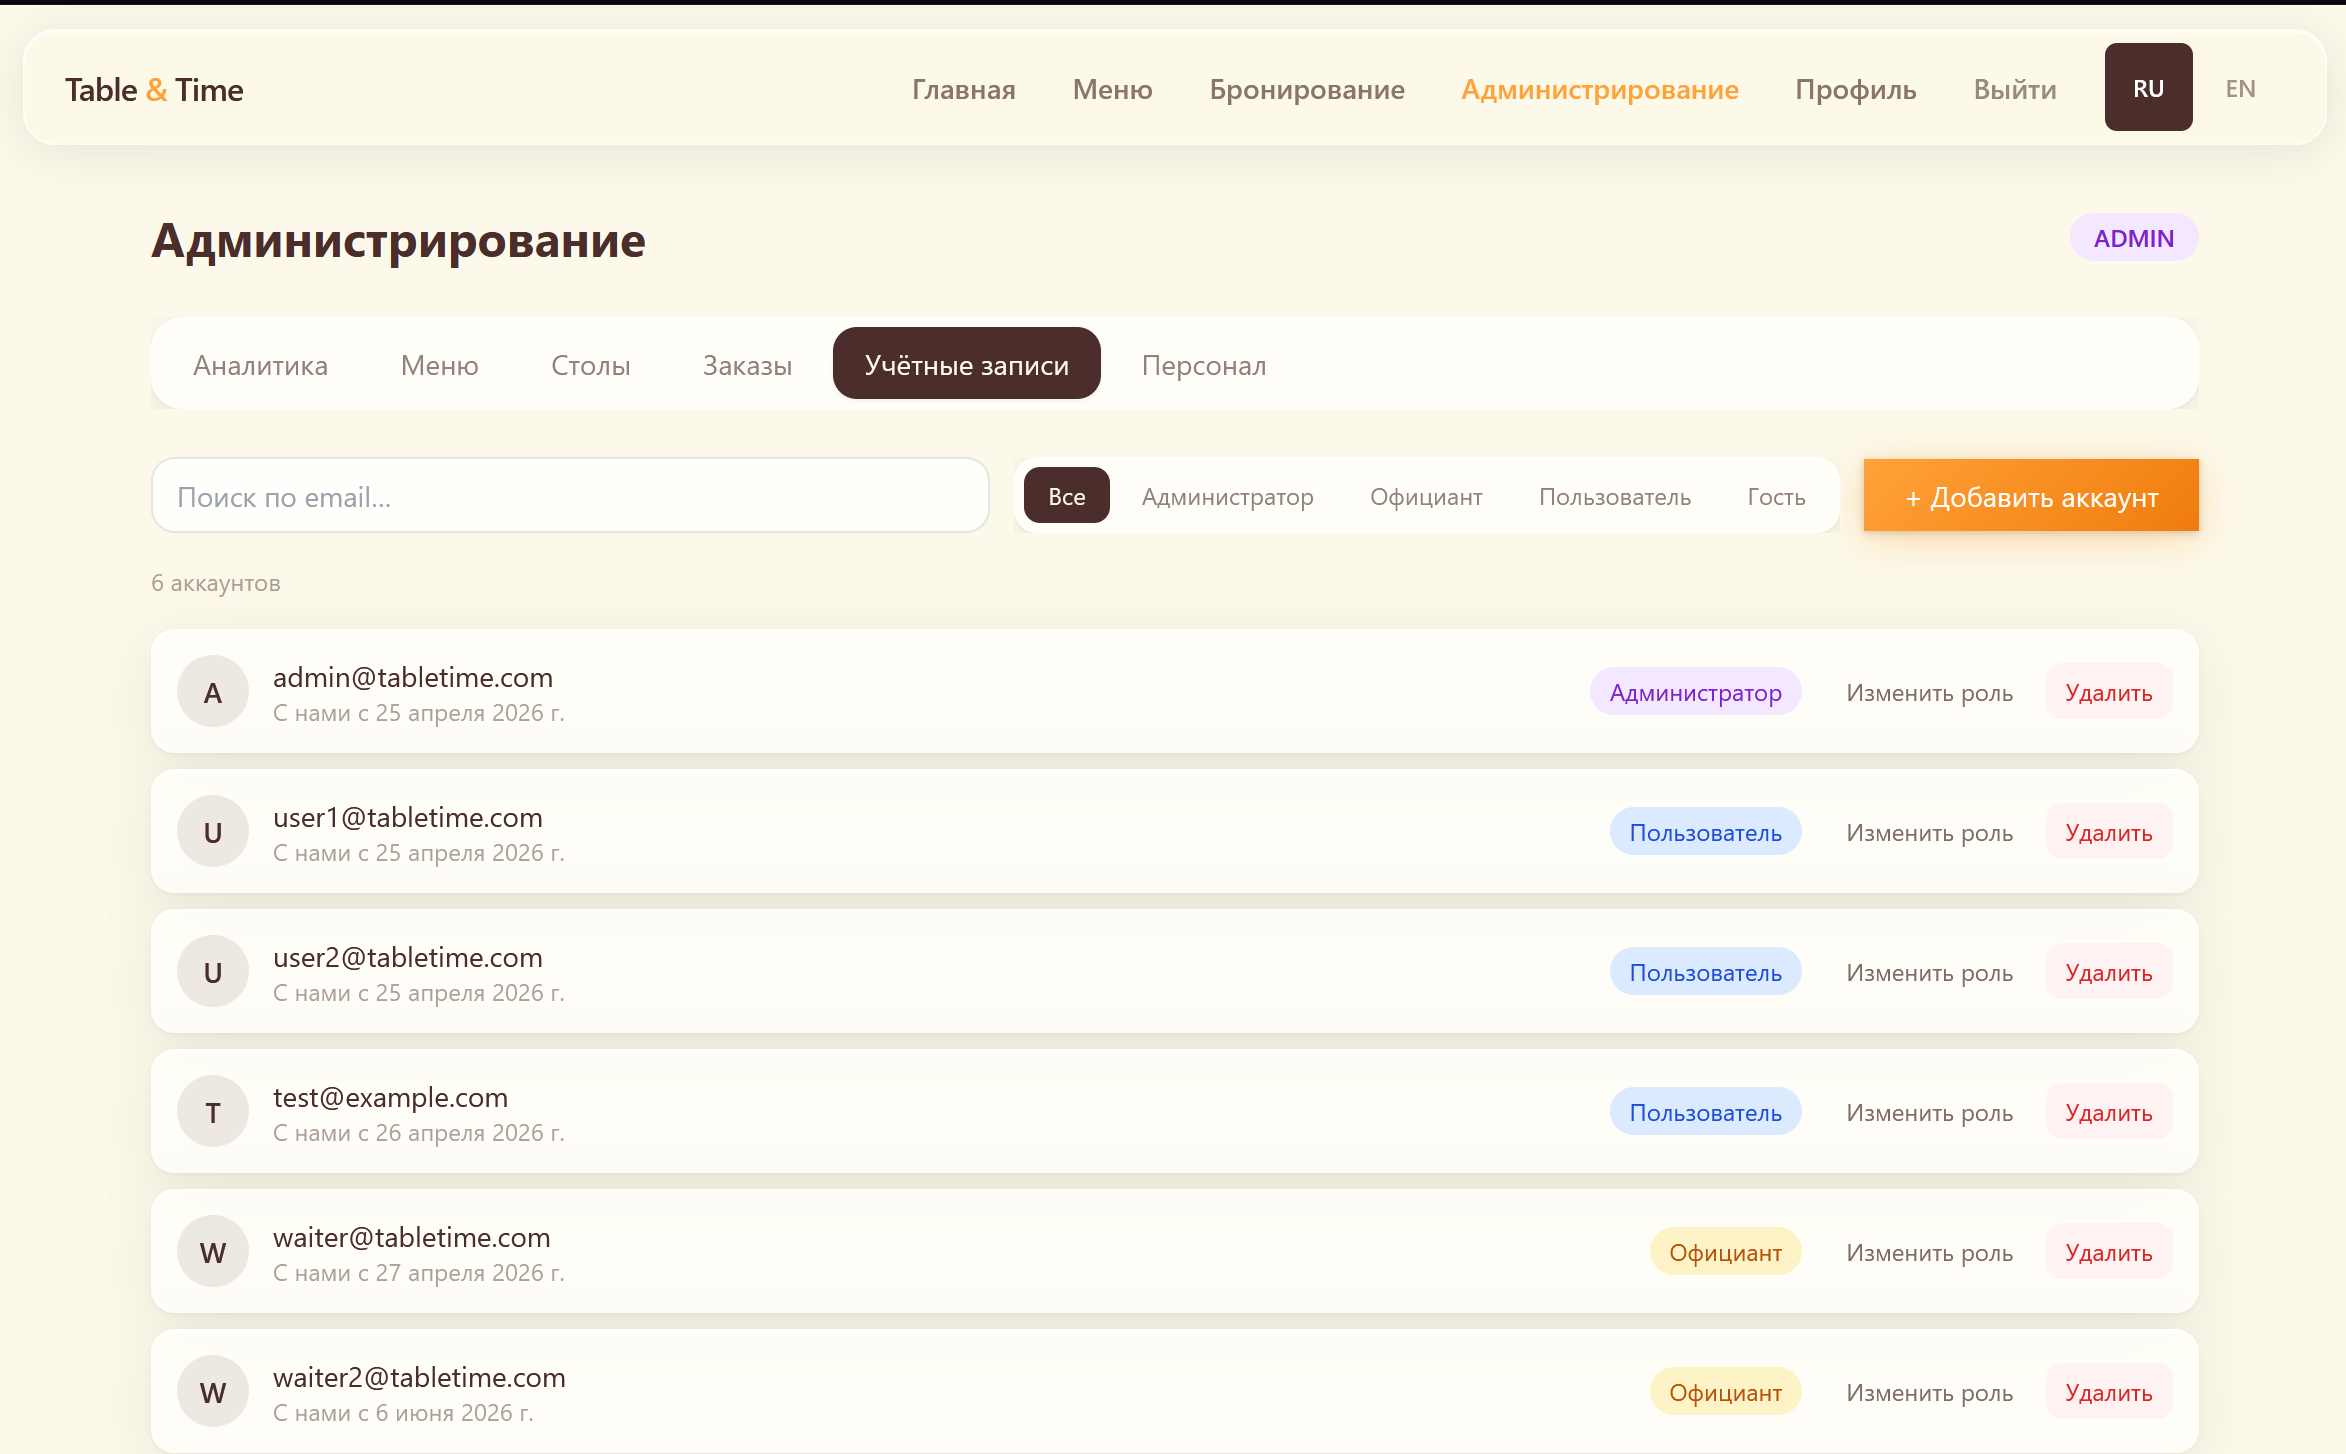
\includegraphics[width=0.85\textwidth]{images/accounts.png}
\caption{Вкладка «Учетные записи»: список пользователей с фильтром по
         роли и форма создания аккаунта}
\label{fig:admin_accounts}
\end{figure}

\subsubsection{Вкладка «Персонал»}

Вкладка персонала отображает карточки всех официантов с указанием
количества назначенных столов, количества выполненных заказов за
текущий день и числа активных заказов. Информация формируется
динамически: завершённые заказы подсчитываются по записям за текущие
сутки, активные~--- по незавершённым заказам за столами официанта.

\begin{figure}[H]
\centering
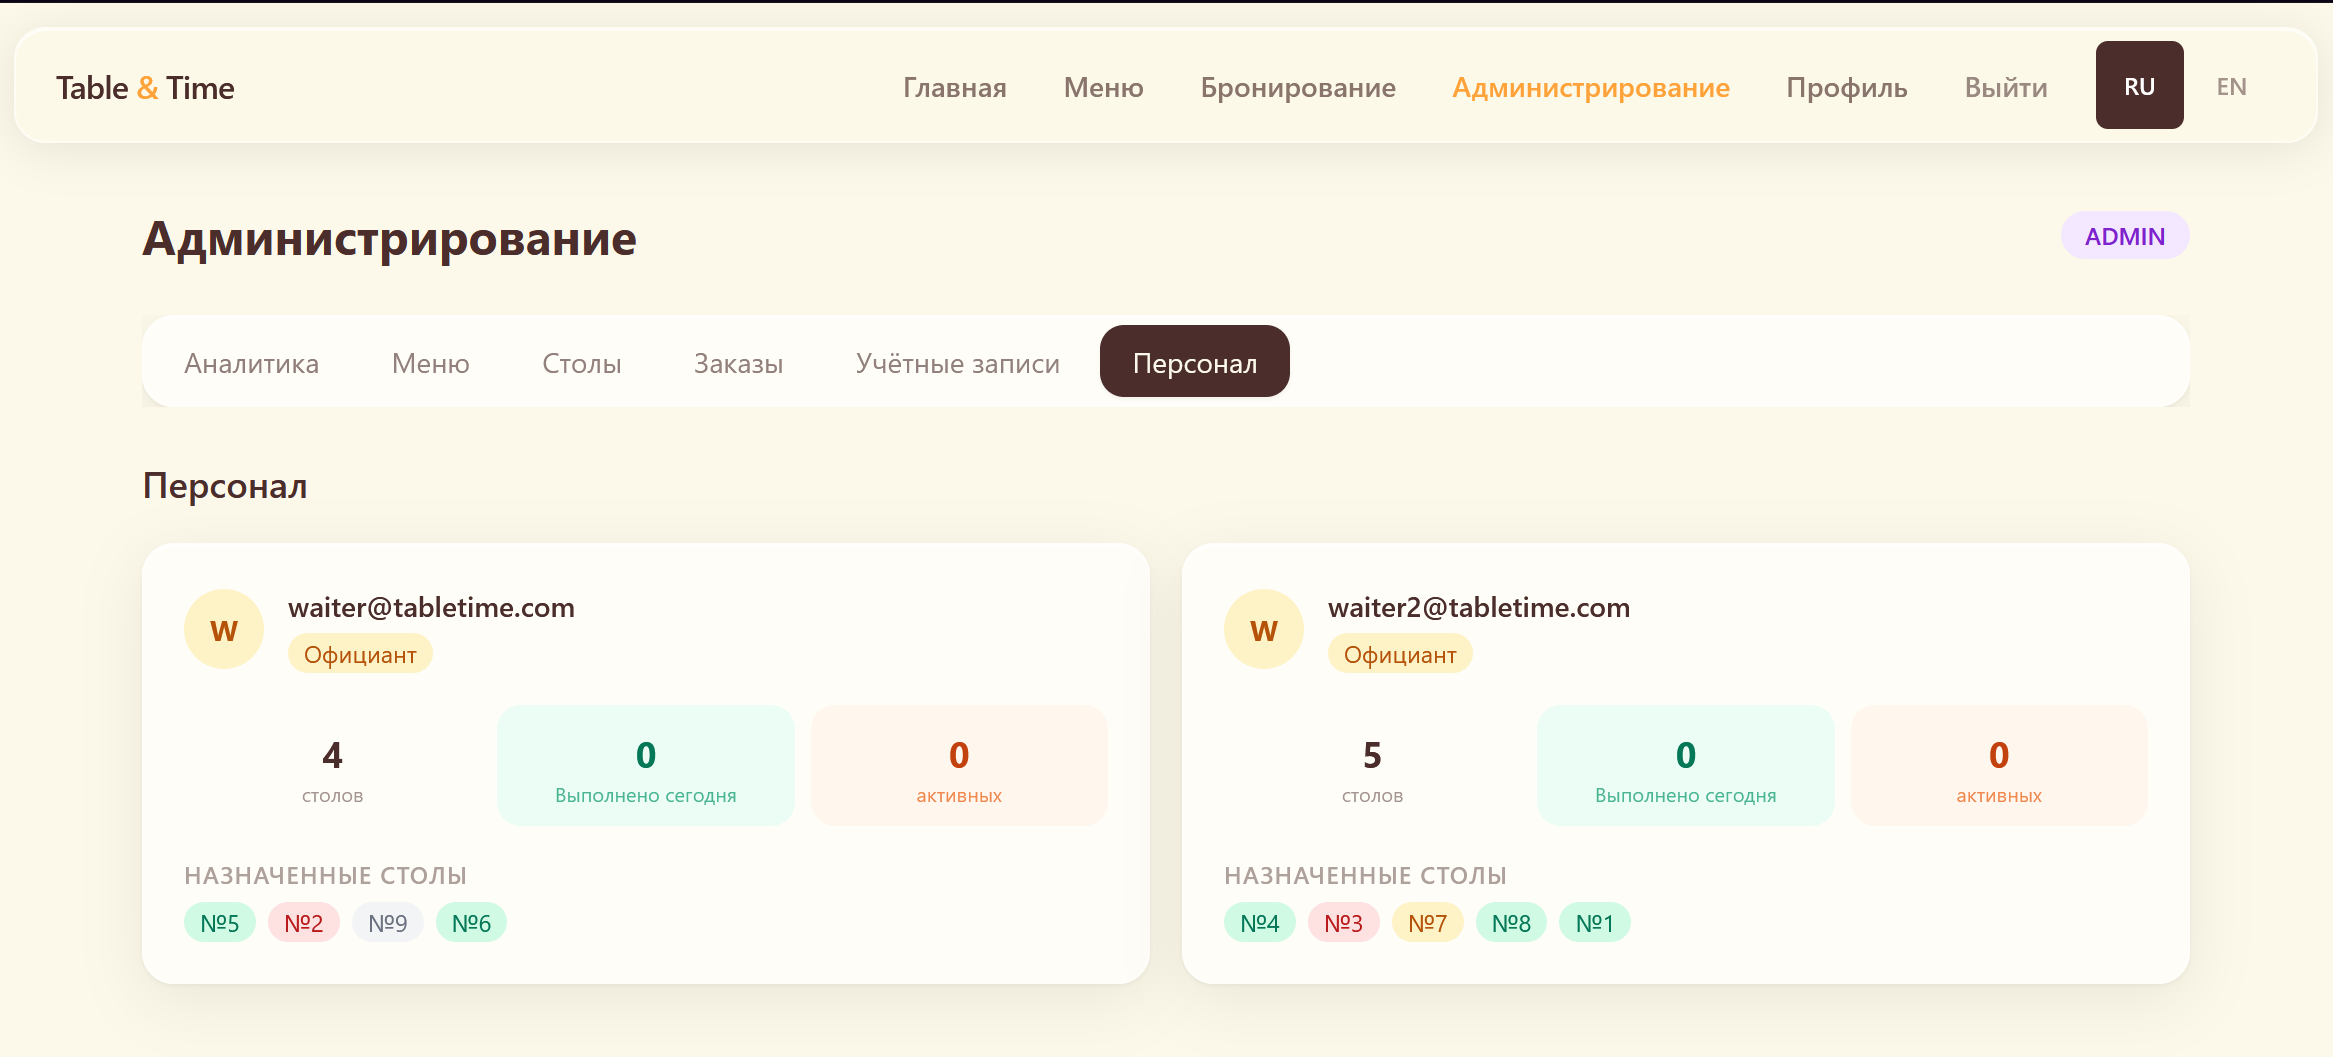
\includegraphics[width=0.85\textwidth]{images/staff.png}
\caption{Вкладка «Персонал»: карточки официантов с количеством
         столов и статистикой заказов}
\label{fig:admin_staff}
\end{figure}

% ----------------------------------------------------------------
\subsection{Проверка работы приложения}
% ----------------------------------------------------------------

После реализации основных функций была выполнена ручная проверка
работы приложения по сценариям для каждой роли пользователей.

Для гостя (\texttt{GUEST}) проверялись:
\begin{itemize}
  \item просмотр главной страницы и меню с переключением категорий;
  \item просмотр карты столов и текущих статусов;
  \item отсутствие доступа к бронированию и оформлению заказов без
        авторизации;
  \item перенаправление на страницу входа при попытке перейти
        к защищённым разделам.
\end{itemize}

Для зарегистрированного пользователя (\texttt{USER}) проверялись:
\begin{itemize}
  \item регистрация и вход в систему;
  \item бронирование стола с указанием даты, времени и количества
        гостей;
  \item отказ системы при попытке забронировать занятый стол на
        текущее время;
  \item успешное бронирование занятого стола на время через два часа;
  \item оформление заказов всех трёх типов;
  \item просмотр истории бронирований и заказов в личном кабинете;
  \item отмена предстоящего бронирования.
\end{itemize}

Для официанта (\texttt{WAITER}) проверялись:
\begin{itemize}
  \item просмотр назначенных столов;
  \item управление статусами заказов (подтверждение, начало
        приготовления, выдача);
  \item отсутствие доступа к административной панели.
\end{itemize}

Для администратора (\texttt{ADMIN}) проверялись:
\begin{itemize}
  \item добавление, редактирование и удаление блюд, изменение их
        доступности;
  \item ручное изменение статуса стола, назначение официанта;
  \item управление статусами заказов;
  \item создание нового аккаунта с указанием роли;
  \item изменение роли существующего пользователя;
  \item просмотр статистики по персоналу.
\end{itemize}

В результате проверки основные функции приложения работают корректно.
Реализованное приложение соответствует требованиям к курсовому
проекту: оно поддерживает аутентификацию и авторизацию с
разграничением прав по ролям, интерактивное бронирование столов с
отображением актуальных статусов в реальном времени, оформление
заказов трёх типов, а также управление меню, персоналом и учётными
записями через административную панель.

% ----------------------------------------------------------------
\subsection{Система контроля версий и структура репозитория}
% ----------------------------------------------------------------

Для хранения исходного кода проекта использовалась распределённая
система контроля версий Git. Удалённый репозиторий размещён на
платформе GitHub по адресу
\url{https://github.com/klimdeliops/Table-time-cafe-app}.
Репозиторий содержит монорепозиторную структуру: в корневой
директории расположены два независимых подпроекта~---
\texttt{backend/} (серверная часть) и \texttt{frontend/}
(клиентская часть), а также общие конфигурационные файлы.

Файл \texttt{.gitignore} настроен таким образом, чтобы исключить
из репозитория директории \texttt{node\_modules/}, артефакты сборки
(\texttt{dist/}, \texttt{.next/}), файлы переменных окружения
(\texttt{.env}, \texttt{.env.local}) и кэш TypeScript
(\texttt{*.tsbuildinfo}). Для каждого из подпроектов созданы файлы
\texttt{.env.example}, содержащие шаблоны всех необходимых
переменных окружения без конфиденциальных значений~--- это позволяет
новому разработчику развернуть проект, не имея доступа к
production-конфигурации.

Ветвление организовано по принципу одной основной ветки \texttt{main},
в которую напрямую вносятся изменения в рамках учебного проекта.
Каждый коммит отражает логически завершённое изменение: добавление
функциональности, исправление ошибки или изменение конфигурации
развёртывания.

% ----------------------------------------------------------------
\subsection{Контейнеризация серверной части с использованием Docker}
% ----------------------------------------------------------------

Серверная часть приложения упакована в Docker-контейнер для
обеспечения воспроизводимости окружения и независимости от среды
хостинга. Конфигурация описана в файле \texttt{backend/Dockerfile}.

В качестве базового образа выбран \texttt{node:20-slim}~---
минималистичная сборка на основе Debian, в отличие от Alpine-варианта
содержащая GNU~libc, что необходимо для корректной работы библиотеки
OpenSSL, используемой Prisma при подключении к базе данных.
Зависимость \texttt{openssl} устанавливается явно через пакетный
менеджер \texttt{apt-get}.

\begin{lstlisting}[language=bash,
                   caption={Dockerfile серверной части},
                   label=lst:dockerfile]
FROM node:20-slim
RUN apt-get update -y && apt-get install -y openssl \
    && rm -rf /var/lib/apt/lists/*
WORKDIR /app
COPY backend/package*.json ./
RUN npm install
COPY backend/ .
RUN ./node_modules/.bin/prisma generate
RUN npm run build
RUN chmod +x start.sh
EXPOSE 3000
CMD ["sh", "start.sh"]
\end{lstlisting}

Используется однослойная (single-stage) сборка, поскольку
многоэтапная сборка с флагом \texttt{--omit=dev} исключила бы
Prisma CLI из итогового образа, что привело бы к ошибке при
выполнении миграций на старте контейнера.

Генерация Prisma-клиента (\texttt{prisma generate}) выполняется на
этапе сборки образа с использованием локально установленного
исполняемого файла (\texttt{./node\_modules/.bin/prisma}) вместо
\texttt{npx prisma}, чтобы исключить автоматическую загрузку
актуальной версии Prisma, которая может быть несовместима с версией,
зафиксированной в \texttt{package.json}.

Запуск контейнера делегирован скрипту \texttt{start.sh}, который
последовательно выполняет три операции: применение накопленных
миграций базы данных, условное начальное заполнение базы данных
(seed) и запуск собранного Node.js-приложения.

\begin{lstlisting}[language=bash,
                   caption={Скрипт запуска контейнера start.sh},
                   label=lst:startsh]
#!/bin/sh
set -e
./node_modules/.bin/prisma migrate deploy
node -e "
  const { PrismaClient } = require('@prisma/client');
  const p = new PrismaClient();
  p.restaurant.count().then(n => {
    p.\$disconnect();
    process.exit(n > 0 ? 0 : 1);
  });
" && echo "Database already seeded, skipping." || npm run seed
node dist/main
\end{lstlisting}

Условие запуска seed-скрипта основано на проверке количества записей
в таблице \texttt{restaurant}: если таблица не пуста, инициализация
пропускается. Это обеспечивает идемпотентность запуска~--- при каждом
перезапуске контейнера пользовательские данные и состояние базы
данных сохраняются.

% ----------------------------------------------------------------
\subsection{Развёртывание и хостинг}
% ----------------------------------------------------------------

Приложение развёрнуто по схеме разделённого хостинга: клиентская и
серверная части размещены на различных платформах, оптимизированных
под соответствующий тип нагрузки.

\textbf{Серверная часть} развёрнута на платформе Railway. Railway
автоматически обнаруживает \texttt{Dockerfile} в репозитории и
выполняет сборку образа при каждом push в ветку \texttt{main}.
Переменные окружения (\texttt{DATABASE\_URL}, \texttt{JWT\_SECRET},
\texttt{ALLOWED\_ORIGINS} и~другие) задаются через панель управления
Railway и передаются в контейнер во время выполнения. База данных
PostgreSQL запущена как отдельный сервис Railway в рамках того же
проекта; строка подключения автоматически инжектируется
в переменную \texttt{DATABASE\_URL}.

\textbf{Клиентская часть} развёрнута на платформе Vercel, которая
нативно поддерживает приложения Next.js и обеспечивает
автоматическую сборку при появлении новых коммитов в репозитории.
Vercel выполняет сборку командой \texttt{next build} и раздаёт
статические ресурсы через глобальную CDN-сеть, что минимизирует
задержку при загрузке страниц. Развёрнутое приложение доступно по
адресу: \url{https://table-time-cafe-app.vercel.app}.

